\documentclass[12pt]{article}
\usepackage{setspace}
\usepackage{amsmath}
\usepackage{bm}
\usepackage{tikz}
\usepackage{graphicx}
\usepackage{float}
\usepackage[margin=1 in]{geometry}
\usepackage{caption}
\usepackage{subcaption}
\usepackage{color}
\usepackage[numbers]{natbib}
\usepackage{amssymb}
\usepackage{algorithm}
%\usepackage[noend]{algpseudocode}
%\usepackage{dirtytalk}
%\usepackage{subfigure}
\usepackage{mathtools}
\usepackage[toc]{appendix}
%\usepackage[titletoc,toc,title]{appendix}
%\usepackage{algpseudocode}
\usepackage{algorithm}
\usepackage{algpseudocode}
\usepackage{listings}
\lstloadlanguages{R}
\usepackage{relsize}
\usepackage{multirow}
\usepackage{titling}
\usepackage{blindtext}
\usepackage{scalerel}
\usepackage{pdfpages}
\usepackage{lscape}
%\doublespacing
\usepackage{color,soul}
\usepackage{siunitx}

\newcommand\floor[1]{\lfloor#1\rfloor}
\newcommand\ceil[1]{\lceil#1\rceil}
\newcommand{\algrule}[1][.2pt]{\par\vskip.5\baselineskip\hrule height #1\par\vskip.5\baselineskip}

\newcommand\vfrac[2]{\ThisStyle{%
  \setbox0=\hbox{$\SavedStyle#1#2$}%
  \setbox2=\hbox{$\SavedStyle X$}%
  \ifdim\ht0>\ht2\setlength{\ht0}{\ht2}\fi%
  #1\mathord{\stretchto{\raisebox{2.3\LMpt}{$\SavedStyle/$}}{\ht0}}#2}}
  
\DeclarePairedDelimiter\abs{\lvert}{\rvert}%
\DeclarePairedDelimiter\norm{\lVert}{\rVert}%

\newtheorem{theorem}{Theorem}
\newtheorem{lemma}{Lemma}
\newtheorem{conj}{Conjecture}
\newtheorem{definition}{Definition}

\newcommand{\beginsupplement}{%
        \setcounter{table}{0}
        \renewcommand{\thetable}{S\arabic{table}}%
        \setcounter{figure}{0}
        \renewcommand{\thefigure}{S\arabic{figure}}%
     }
     

\title{Meta Quantile Regression: A Novel Method for Detecting Potential Gene Interactions using Sample Distributions of Complex Traits}

\author{Akram Alyass$^*$, Arkan Abadi$^*$, Ben Bolker, David Meyre}


\begin{document}
\setcounter{secnumdepth}{0} %% no numbering

\begin{titlingpage}
    \maketitle
    \begin{abstract}
\underline{\textbf{Background}}: The effect of genetic variants on complex traits includes interaction components that are challenging to reliably detect. Meta-Quantile Regression (MQR) is a framework that combines conditional quantile regression (CQR) and meta-regression to infer potential interactions by modeling variations in genetic effects across the sample distribution of quantitative traits. 

\underline{\textbf{Objectives}}: Compare the utility of MQR and variance heterogeneity tests for detecting potential interactions. 

\underline{\textbf{Methods}}: The relationships between variance per genotype and MQR were analytically investigated. MQR fitted using CQR were termed as MCQR to differentiate them from MQR models fitted using unconditional quantile regression (UQR) which were termed as MUQR. The computational cost and asymptotic convergence rate of MCQR and MUQR estimates were compared using simulations.  Variance heterogeneity tests investigated include Levene's and Brown-Forsythe \textit{F}-tests for a total of 4 tests of potential interactions (Levene, Brown-Forsythe, MCQR, and MUQR). Simulations were conducted to compare their type I error and power by 1) the number of genotype group levels; 2) symmetric, asymmetric error, and inverse-normal rank transformation to treat skewness; and 3) synergistic and antagonistic interactions. 

\underline{\textbf{Results}} QR estimates were analytically shown to be influenced by unadjusted interactions that capture the change in distribution spread by genotypes. MUQR models were found to use less CPU time to fit and provide estimates that asymptotically converge faster than MCQR models. Furthermore, rank-transformations were shown to inflate type I error rates for 4 four tests on genotypes with main effects. Both MCQR and MUQR were found to have higher power of detecting potential interactions with the number of genotype group levels; under asymmetric error, and antagonistic interactions compared to variance heterogeneity tests. 

\underline{\textbf{Conclusions}}: MQR models are useful for identifying potential interactions and MUQR is a computationally feasible framework for genome-wide association studies.

    \end{abstract}
\end{titlingpage}
 
\section{Introduction}
\indent \indent Complex traits are influenced by a combination of environmental and genetic components. Over the past decade, a growing number of genetic variants have been associated with complex traits using genome-wide association studies (GWAS) \cite{wood2014defining, locke2015genetic, global2013discovery}. While GWAS has been effective for uncovering variants that are directly associated with such traits, the role of genetic interactions (e.g. gene$\times$gene / gene$\times$environment) remains unresolved. Identifying genetic interactions is important for elucidating the genetic architecture and biological networks that underlie complex traits. Gene interactions refer to circumstances where an interacting variable modifies the effects of a genetic variant on a phenotype. Interacting variables could be other genetic variants (i.e. epistasis), environmental (e.g. pollutants), biological (e.g. sex or age), behavioral exposures (e.g. smoking or unhealthy eating) or medical conditions (e.g. chronic diseases). Genome-wide interaction study (GWIS) designs typically incorporate interaction terms in a regression framework to identify gene interactions.  However, accurate and reliable measurement of environmental exposures remains an area of active investigation \cite{reddon2016physical}. For example, collecting dietary intake data that is representative of real behavior has methodological limitations and as a result, few GWIS have been successful in identifying interactions \cite{grandjean2012dietary, risch2009interaction, scott2012no, culverhouse2017collaborative}. There is a need for robust statistical methods to detect gene interactions at a more general level that do not rely on measurements of presumed interacting variables. Such methods identify loci with potential gene interactions but would not confer the source (e.g. unmeasured diet or physical activity levels) or nature (e.g multiplicative or threshold-based) of these interactions. This would cue follow-up investigations without limiting the scope of explorations to single source and nature of interaction. 

Differences in phenotype variance across genotypes have recently gained attention as a potential statistic for detecting interactions \cite{struchalin2010variance, sun2013significance, pare2010use,gauderman2013finding}. For example, if a bi-allelic genetic variant (e.g. single nucleotide polymorphisms - SNPs) interacts with physical activity to affect BMI, then the variability in BMI will be higher in subjects carrying the BMI-increasing allele given that a portion of carriers will engage in some level of physical activity. Hence, testing for differences in variance across genotype categories can provide evidence of gene interactions. However, variance  is not the only measure of a distribution's spread and it is possible for phenotype distributions to have similar variances across genotypes but different interquartile ranges, minimum and maximum values by genotype. Many phenotypes of interest have heavy-tailed distributions (e.g. BMI, plasma glucose, or protein expression data) for which the mean and variance are not necessarily the best measurements of location and shape. An alternative approach to capture differences between distributions by genotype is to model the effect of variants across the sample distribution using quantile regression (QR) \cite{koenker1978regression}. This is based on the principle that gene interactions induce differences in the marginal effects of genetic loci across quantiles of a trait  \cite{abadi2017penetrance, koenker1982robust}. First degree differences in QR estimates across quantiles denote changes in distribution spread that are essentially quantile-widening effects \cite{koenker1982robust}. Meta-regression can be used to model such quantile-widening effects which are analogous to heteroscedasticity tests \cite{koenker1982robust, abadi2017penetrance}. We term this framework Meta-Quantile Regression (MQR) and we have implemented it to identify potential gene interactions without knowledge of the interacting variable(s)\cite{abadi2017penetrance}. 

The computational cost of fitting CQR models can be prohibitive at scale because estimates require optimizations. In addition, the asymptotic variance-covariance matrix of estimates is challenging to evaluate because it depends on an unknown response density. Bootstrapping methods are required to reliably estimate the variance-covariance matrix, which limits the utility of QR methods in genome-wide analysis \cite{hagemann2017cluster}. We used unconditional quantile regression (UQR) to overcome the challenges of CQR and identify variants with potential interactions \cite{firpo2009unconditional}. Importantly, marginal effects can be correlated with quantile-widening in the absence of gene interactions, and this phenomenon is commonly referred to as scaling (i.e mean-variance correlations). We formulate a framework to adjust quantile-widening effects for scaling so that potential gene interactions are no longer confounded. Simulations to assess type I error and the power to detect potential interactions compared with variance heterogeneity tests were also performed. An emperical analysis of ~31,000 SNPs in 71,230 participants of European descent was also conducted to detect potential gene interactions on BMI. 

\section{Materials and Methods}

\subsection{Simulations} 
\paragraph{Data Generation}Assume the following linear model
\begin{equation} \label{mod1}
y_i = \beta_0 + \beta_1 x_i + \beta_2 g_i + \beta_3 x_i g_i + \epsilon_i
\end{equation}
where $x_i$ corresponds to an interacting variable with $X \sim F_X (\mu_x,\sigma_x^2)$; $g_i$ is the observed genotype of the genetic variant, $G$, under HWE with the population allele frequency, $p$, where $G \sim Bin(2, p)$; and $\epsilon_i$ is the random error with $\epsilon \sim F_{\epsilon} (0, \sigma_\epsilon)$. $\beta_0$, $\beta_1$, $\beta_2$ and $\beta_3$ correspond to the intercept, marginal effect of the interacting variable, marginal effect of the genotype, and the interaction effect between them, respectively. Genotypes were generated from $\text{Bin}(\eta, p)$ centered at $\mu_g =0$ with $\sigma_g = \eta p(1-p)$, where $\eta$ is one plus the number of chromosomes (i.e. $\eta=2$ for two levels of an indicator for whether the single chromosome contains the reference allele) and $p$ is the allele frequency. For simplicity, genotypes are generated from $\eta=2$, unless otherwise specified. Genotypes were investigated under an additive genetic effect with allele frequencies ranging from $0.05$ to $0.95$. The interacting variable $X$ was generated from a standard normal distirbution. The response variable, $Y$, was simulated from the linear model in equation \ref{mod1}. Coefficients of individual covariates were calculated as a function of pre-defined \% variance explained ($R^{2}$) by individual marginal and interaction variables denoted as $R^{2}_G$, $R^{2}_X$, and $R^{2}_{G \times X}$. Regression coefficients were specified as $\beta_0=0$, $\beta_1 = \sqrt{R^{2}_X}$, $\beta_2 = \sqrt{\vfrac{R^{2}_G}{\big(\eta p(1-p)\big)}}$, and $\beta_3 = \sqrt{\vfrac{R^{2}_{G \times X}}{\big(\eta p(1-p)\big)}}$ unless otherwise specified \cite{pare2010use, gauderman2013finding}. The random error $\epsilon$ was simulated from skew-normal distribution with mean zero and and variance equal to $1 - R^{2}_G - R^{2}_X - R^{2}_{G \times X}$. The error was simulated with shape parameters $\alpha_{\epsilon}=  0$ and $20$ to denote symmetric and asymetric distributions respectively. The treatment of skewness using rank-based inverse-normal transformation were also assessed. The variance explained by the interacting variable $X$ was fixed at $R^{2}_X = 24\%$ for all simulations while $R^{2}_G$ and $R^{2}_{G \times X}$ were varied from $0$ to $0.4\%$. A total of $R=10,000$ replications were performed for all simulated datasets with each having a sample size of $n=10,000$ independent observations. Both sample size and percent variance explained by genetic variants realistic in the context of GWAS and GWIS \cite{wang2015review}.

We investigated conditions that induce correlations between estimates of marginal and quantile-widening effects, commonly known as scaling phenomena. 1) Scaling due to error skewness, termed 'pseudo-scale effects', which is analogous to skewed random error term described above for asymetric distributions. The random error $\epsilon$ sampled from an exponential distribution (rate=0.1) that was scaled to have a mean equal to zero and variance equal to $1 - R^{2}_G - R^{2}_X - R^{2}_{G \times X}$. 2) Scaling due to linear heteroscedasticity as a function of marginal effects, termed 'true-scale effects'. Given a simple linear model with a heteroscedasticity function, the conditional variance of $Y$ can be shown to be
\begin{equation} \label{TrueScaleMod}
Var(Y|G=g)=\sigma_x^2 (\beta_1+\beta_3 g)^2 + \sigma_\epsilon^2 (1+\gamma\beta_2 g)^2
\end{equation}
where $\gamma$ is the true scaling effect parameter due to genotype marginal effects $\beta_2$. This type of scaling effect can occur in symmetric and asymmetric distributions. As such, we define $R^{2}_{G\: Total} = R^{2}_{G} (1+\gamma)$ to denote the total variance explained by the marginal effect, where $R^{2}_{G}$ is computed as described above and $\gamma=0.1$. The residual variance under a true-scale effect is computed as $1 - R^{2}_{G\: Total} - R^{2}_X - R^{2}_{G \times X}$. 3) Rank-based scale effects correspond to scale effects as a function of sample rank. Here, the outcome distribution for sample $y_i$ was linearly amplified such that $y_i^\star=y_i(1 + \tau \omega)$, where $\tau$ is the percentile rank, and $\omega=0.5$ is the rank-multiplier. Additional details explaining these types of scaling is presented in the supplementary materials. These types of coerced correlations encompass the challenges of investigating quantile-widening effects for variables with marginal effects on the response. 

\paragraph{Test Statistics} Tests for equality in variance by genotype included Levene's mean-based F-test, and the Brown-Forsythe F-test \cite{struchalin2010variance}. Test statistics for quantile-widening effects, detailed in the supplementary methods, entail fitting a linear model on the QR estimates across the sample distribution percentiles. Scaling effects denote a proportionality between marginal and quantile-widening effects, therefore it is reasonable to model this relationship using a regression approach {Young:2018ej}. The goal is to decompose quantile-widening effects that are attributed to marginal effects (i.e. scaling) from quantile-widening effects that are attributed to potential interactions. For simplicity, we assume additive linear scale effects and model scaling using robust regression (median regression) weighted by the \textcolor{red}{double check this : inverse-variance of marginal effects}. This scaling model can then be used to predict the quantile-widening effects from the marginal effects of SNPs (i.e. the quantile-widening effects predicted by scaling alone). The estimated quantile-widening effects of each SNP can then be adjusted using the scaling model according to their marginal effects. The scaling-adjusted quantile-widening effect and corresponding standard errors are given by
\begin{equation}
\begin{split}
\hat{\beta}_{MR_{adj}}&=\hat{\beta}_{MR} - \hat{\beta}_{SM} \\
s.e(\hat{\beta}_{MR_{adj}}) &= \sqrt{s.e(\hat{\beta}_MR)^2 + s.e(\hat{\beta}_{SM})^2}
\end{split}
\end{equation}
where $\hat{\beta}_{SM}$ is the predicted variance effect given mean effects.

\paragraph{Type I Error}Type I error rates for individual tests were computed as the proportion of false positives of $R=10,000$ replications at a nominal level of $0.05$. False positive rates were assessed while varying the symmetry of error distribution (symmetric or asymmetric), and on rank-based inverse normal transformation of the asymmetric error (i.e. skewed response variable). $R^{2}_{G}$ was varied between $0\%$ and $0.4\%$. All $p$, $R^{2}_{X}$ and $R^{2}_{G \times X}$ were fixed at $5\%$, $24\%$ and $0\%$, respectively. The false positive rate of unadjusted UQR for marginal effects of $G$ was also provided to demonstrate the effect of mixtures of marginal and interaction effects on trends of $\beta_G (\tau)$ with $\tau$ for UQR. A direct interaction test using CQR is also applied as a reference for other tests. 

\paragraph{Power to Detect Associations}The power of each test for detecting potential interactions was computed as the proportion of replications that correctly reject the null hypothesis at a nominal significance level of $\alpha=0.05$. Power was computed to assess the impact of 1) the number of genotype levels, 2) skewness, and 3) antagonistic interactions on the ability of variance heterogeneity tests (Levene's F-test, and BF test) and MQR-based tests (MCQR, MUQR) to detect a single unadjusted two-way interaction. The number of genotype levels was varied from 2 (i.e. single chromosome) to 5 levels (i.e. 4 chromosomes) where allele frequency is varied from $0.05$ to $0.95$.  The effect of skewness on power was assessed by varying error distribution (symmetric, or asymmetric), and $R^{2}_{G \times X}$ ($0\%$ to $0.4\%$). The effect of antagonistic interaction effects was assessed similarly, but with an interaction coefficient having opposite direction compared to main effect of the interacting variable. The main effect of the interacting variable is set to be positive, while the coefficient for interaction effect is negative to correspond to antagonistic interaction effects.

\subsection{Empirical Analysis}
\indent \indent Studies listed on the database of phenotypes and genotypes (dbGaP) were identified for whom individual-level genotype and BMI data were available. After obtaining local ethics committee (Hamilton Integrated Research Ethics Board-HiREB) approval and study-specific access approval, a total of 14 studies were selected for further analysis. These were ARIC (phs000280.v3.p1), CARDIA (phs000285.v3.p2), CHS (phs000287.v6.p1), the Framingham cohort (phs000007.v29.p10), MESA (phs000209.v13.p3), COPD (phs000179.v5.p2), BEAGESS (phs000869.v1.p1), GARNET (phs000343.v3.p1), HABC (phs000169.v1.p1), NHS/HPFS (phs000091.v2.p1), NESDA (phs000486.v1.p1) , PGRN-RIKEN (phs000331.v1.p1) and the WHI (phs000200.v10.p3). In addition, genotype and phenotype data from one local study EpiDREAM was also included in the analysis \cite{Gerstein:2004ek}. Measurements collected from participants below age 18 or above the age of 92 were excluded ($<$1\%). For studies with repeated measures across multiple time points or visits, the median height and the median weight was extracted along with the corresponding age at these median values. BMI was calculated by dividing the median weight (kg) by the square of the average measures of height (m). Analyses were restricted to participants of European ancestry (EA, self-reported) with a combined sample size of 71,230. All analyses are consistent with study-specific Data Use Certifications (DUC).

Sample Quality Control (QC): Detailed genotyping procedures for EpiDREAM and studies from the Candidate Gene Association Resource (CARe) project including, ARIC (phs000557.v2.p1), CARDIA (phs000613.v1.p2), CHS (phs000377.v4.p1), the Framingham Cohort (phs000282.v17.p10) and MESA (phs000283.v7.p3) are presented elsewhere \cite{anand2012glucose, musunuru2010candidate}. Genotyping was performed using the gene centric HumanCVD Genotyping BeadChip with 49,320 markers concentrated in $~$ 2,100 loci that are related to metabolism and cardiovascular disease.{Keating:2008kc}



%A detailed description of the studies, participants, sample and marker quality control, marker imputation procedures are presented in the supplementary files. Briefly, studies on database of phenotypes and genotypes (dbGaP) for whom individual-level genotype and BMI data were available were identified. After obtaining local ethics approval and study-specific access approval, a total of 18 studies were selected for further analysis. In addition, genotype and and phenotype data from one local study EpiDREAM was also included in the analysis. 

\section{Results}
\subsection{Simulations} \textcolor{red}{consider removing much of the levene because it is already known adds nothing to include it}
Figure ~\ref{fig:FP} shows Type I error rates for test statistics under symmetric and asymmetric errors with and without rank-based inverse-normal transformation when $R^{2}_G= 0\%$ and $04\%$. Levene's F-test showed an increased Type I error rate for asymmetric error in comparison to BF F-test that was near nominal. MCQR showed a slightly elevated Type I error rate that was stable across the scenarios investigated. This results from the range and the number of percentiles considered which produced slight deviations from normality (Figure \ref{fig:FS1}) \textcolor{red}{[this was done with iid redo it with mcmb]}. In addition, MUQR unadjusted for genotype effects had an increased Type 1 error rate resulting from marginal and interaction effects of $G$ as discussed in the supplementary \textcolor{red}{move to supplementary}. Adjusting for the marginal genotype effect resulted in a near nominal level of false positives for UQR\textcolor{red}{move to supplementary}. Rank-based inverse-normal transformation of response variables with skewed error resulted in increased Type I error rates for all test of variants with non-zero marginal effects. 

Figures \ref{fig:PowLevel} and \ref{fig:PowLevel45} show the power of detecting potential interactions with increasing number of group levels (e.g. mono, bi, tri, and quad allelic genotypes). MCQR and MUQR show higher power compared to variance heterogeneity tests when there are more than two genotype levels \ref{fig:PowLevel45}. This can be explained by the fact that variance heterogeneity relies on subgroup analysis for variance per-genotype whereas MCQR and MUQR utilize the whole sample to compute the test statistic \textcolor{red}{move to discussion}. The power remains constant across allele frequency because the variance explained by interactions is maintained at $R^{2}_{G \times X}=0.1\%$). Figure \ref{fig:Pow1} shows the power of detecting potential synergistic and antagonistic interactions under both symmetric ($\alpha_\epsilon = 0$) and asymmetric ($\alpha_\epsilon = 20$) error distributions for bi-allelic genotypes. Under symmetric error distribution, MCQR and MUQR showed higher power of detecting interactions compared to variance heterogeneity tests due to the genotype group level described earlier. However, this difference in power increased greatly under an asymmetric error distribution. This is due to the sensitivity of variance estimates to skewness that increases their sampling error for skewed distributions \cite{lee1998testing}. \textcolor{red}{consider adding stuff from toronto team, when error is skewed they add transformation, but adjust for main effect, double check on power for antagonistic interactions when transformed and adjusted with simulation of our own} In contrast, MCQR and MUQR are not affected by skewness because they rely on distribution quantiles. The power of all four tests was redced under antagonistic interactions, but the power of MQR based tests decreased less than variance heterogeneity tests. This difference is even larger under asymmetric error distributions \textcolor{red}{this may need to be re-written when we redo simulations plus testing indicating}. 

\paragraph{Scaling Effect Adjustments} Investigating quantile-widening effects (or variance heterogeneity effects) when marginal effects and response skewness are present can be complicated by scaling effects. Scaling effects produce correlations between marginal effects and quantile-effects and can therefore lead to spurious findings if not properly addressed. We investigated scaling effects under three different conditions including (1) pseudo-scaling, i.e. skewed error distribution; (2) true-scaling, i.e. heteroscedasticity as a function of marginal effects; and (3) rank-based scaling, i.e. scale effects as a function of sample rank \ref{fig:ScaleEffTypes}. Figure \textcolor{red}{wrong figure} \ref{fig:ScaleEffPower} summarizes the false positive rate under different types of scale relationships. All three types of scaling effects increased the false positive rate. As expected, inverse-normal rank-transformation, reversed the increased false positive rate under rank-scaling effects but markedly increased the false positive rate for pseudo-scaling. This suggests that without knowing the nature of the scaling effect, inverse-normal rank-transformation should be applied with caution when studying gene interactions. \ref{fig:ScaleEffPower} shows that adjusting for scaling effects effectively restores the false positive rate to nominal levels under all types of scaling. In addition, \ref{fig:ScaleEffPower} shows that the power to detect gene interactions can be largely maintained after adjusting for scaling effects. As noted earlier with asymmetric error, the power of detecting interactions under pseudo-scaling is increased. Adjusting for scaling under conditions of true-scaling effects did not affect the power to detect gene interactions, while adjusting for scaling under rank-based scaling effects did decrease the power to detect gene interactions slightly. 

\subsection{Empirical Analysis}
We investigated evidence of potential interactions for SNPs represented CVD array with BMI. After removing rare variants (MAF $<$5\%) and variants with genotypes in fewer than 30,000 participants; 30,995 variants remained \ref{fig:ManhattanPlots}. 24 and 18 SNPs showed significant quantile-widening effects after adjusting for multiple testing correction (p $<$ \num{1.613E-06}) using MCQR and MUQR, respectively \ref{fig:Table_1_EmpiricalResults}. 17 and 14 of these were significant at genome-wide thresholds (p $<$ \num{5E-08}), respectively. 2 SNPs passed the multiple testing correction threshold using MUQR and not MCQR, conversely 8 SNPs passed this threshold with MCQR but not MUQR. The results using MCQR and MUQR were generally similar, although MCQR was more sensitive than MUQR, with respect to power, which is consistent with results from simulations. As expected, SNPs in \textit{FTO} and \textit{GIPR} showed strong variance effects \cite{abadi2017penetrance,Young:2018ej}. These SNPs also have well-established marginal effects on BMI and thus their quantile-widening effects may be explained by scaling. Interestingly, SNPs in \textit{DDAH1} (rs1006988, rs1006989, rs17388437 and rs1146383), \textit{LCT} (rs1042712), \textit{GNAI2} (rs9852677), \textit{RANB17} (rs2053682), \textit{IRAK3} (rs17826057) do not have detectable main effects on BMI but do have detectable quantile-widening effects. A scaling model was fitted to assess the relationship between marginal effects and quantile-widening effects across all SNPs. Scaling-adjusted quantile-widening effects were then computed from this scaling model to isolate the component of the quantile-widening effects that is attributable to marginal effects. The quantile-widening effects of SNPs in \textit{FTO} were largely attributable to their marginal effects ($>$75\%) and scaling-adjusted quantile-widening effects of these SNPs were small. For SNPs in GIPR, approximately 50\% of the quantile-widening effect was due to marginal effects but the scaling-adjusted quantile-widening effects persisted at a nominal level of significance (p$<$0.01) which is consistent with recent reports.\cite{Young:2018ej} As the remaining SNPs did not have detectable marginal effects on BMI, scaling did not account for an appreciable proportion of their quantile-widening effects. In addition because these SNPs had no detectable marginal effects scaling adjustment only served to inflate the error of the quantile-widening estimate.

%(rs8047395, rs1421085, rs9923147, rs17817288, rs1121980, rs7193144, rs17817449, rs11075987, rs3751812, rs11075989, rs9939609, rs7185735, rs9941349, rs9922708, rs12149832, rs11642841)
%(rs11672660, rs10423928)

\section{Discussion}
% Importance of estimates and what we have done
This study expands the application of MQR to detect evidence of potential interactions in the context of genetic association analysis. We show that using MR to model heterogeneity of QR estimates across an outcome distribution is a robust and powerful approach for detecting potential interactions. We show that MUQR overcomes the computational limitation of MCQR. UQR was 2.5-8.5 times faster than CQR via Frisch-Newton approach after preprocessing. Hence, MUQR is more practical for large-scale genome-wide association analyses. MQR methods were also shown to maintain nominal Type I error rate and achieved greater power when compared to variance heterogeneity tests with increasing number of group levels, asymmetric error distributions, and antagonistic interactions. 

This study shows how the shape of QR estimates captures information on the quantile density function of interaction variable(s) (Figure \ref{fig:MotExample}). Fitting MR models on QR estimates using re-centered percentiles around the median allows for estimation of 1) an intercept parameter that corresponds to the marginal effect of genotypes, and 2) a slope parameter that corresponds to the mean change in QR estimates with one-unit change in percentiles and denotes the presence of potential interactions. The effect of SNPs across the sample distribution is a function of error quantiles that assume the same density of the interacting variable(s) (Equation \ref{firstQR}). In the case of a single interaction variable, the quantile function of a univariable error density is increasing by definition. In the case of multiple interacting variables, the quantile function of a multivariate error density is equivariant and thus not strictly increasing in a linear fashion (Supplementary Material) \cite{small1990survey, serfling2008mahalanobis}. Identifying the best model to fit QR estimates across percentiles can, however, be challenging in the context of genome-wide analysis. Assuming a linear trend provides a simple analog of correlation, which implies associations while acknowledging that more complex relationships (i.e. multiple interacting variables with certain types of non-increasing quantile functions) may not be detected given the limited robustness of linear models for detecting non-linear relationships. The approach follows merely the natural association analysis using linear regression in which correlation implies association but not causation, while acknowledging that causation implies association but not correlation \cite{altman2015points}. 

Heteroscedasticity resulting from gene interactions have been characterized previously, where testing for differences in variance per genotype was proposed as an indicator of potential interactions \cite{struchalin2010variance,pare2010use}. Two well-known tests for variance heterogeneity include Levene's F-test and the Brown and Forsythe test \cite{levene1960robust, brown1974robust}. Brown and Forsythe highlighted that Levene's statistic is not robust when the underlying population distribution is skewed and proposed additional treatments to address this problem \cite{brown1974robust}. However, variance as a measure of distribution spread is less informative when applied to skewed phenotypes. As such, variance heterogeneity tests are prone to higher Type I error rates (in the case of Levene's F-test) and have decreased power of detecting differences in distribution spread for skewed distributions as confirmed by Figure \ref{fig:Pow1}. This is because the confidence intervals for variance estimates are larger for skewed distributions \cite{lee1998testing}. Instead, modeling distribution quantiles using QR is more suitable for testing differences in the distribution spread for asymmetric phenotypes by genotype levels. Many biological traits are skewed including those that are harmful at low quantities but tolerated at high quantities (i.e. right skewed blood glucose measures, or BMI) or vice versa. 

Irrespective of trait distribution shape, marginal effects can be subject to scale effects that tie marginal effects to variance effects. Such scaling can complicate the detection of gene interactions because variance effects may be attributed to marginal effects rather than interaction effects. We investigated 3 different types of scaling which we termed pseudo-scale effects, true-scale effects and rank-scale effects; and demonstrated that they could be effectively adjusted for by fitting a regression model. In addition, we showed that traditional methods (log- and rank-based inverse-normal transformations) to address scaling need to be applied with caution when investigating interactions as they may exacerbate the correlation between marginal and variance effects. Specifically, rank-based inverse-normal transformations strengthened scale effects under pseudo-scaling, had no effect on true-scaling, and reversed rank-based scaling. Interestingly, applying rank-based inverse-normal transformation to BMI reduced much of the scaling effect, suggesting that some form of rank-scaling may exist in BMI.

Location-scale-shift models of QR estimates to assess differences in distribution by regressors have been previously proposed \cite{khmaladze1982martingale, koenker2002inference, aschard2013nonparametric}. These approaches enable inference on global differences between distributions by genotype but do not compare location and scale shifts separately. This problem is shared by other non-parametric tests such as Kolmogorov-Smirnov test and other derivatives \cite{massey1951kolmogorov, hart2001mann}. Current quantile-based tests rely on computed reference null distributions (i.e. permutations) that provide p-values with 4 or less significant digits or, else, require approximations of extreme distribution tails \cite{knijnenburg2009fewer}. To our knowledge, there are currently no quantile-based tests that exclusively focus on differences in scale shifts. Hence, MQR as first utilized by Abadi et al. 2017 and elaborated further here in this study, is the first to reliably and efficiently enable robust statistical inference on scale differences \cite{abadi2017penetrance}. It allows for the objective modeling of scale change with genotypes (i.e. linear heteroscedasticity due to one or multiple two-way interactions) as well as more complex terms. Its utility may not only be limited to genetics but to research at large as it provides estimates of both marginal and potential interaction effects. MQR is not restricted to genetic epidemiology alone in the pursuit of precision medicine but applies to all research fields alike. 

This study includes simulations to compare the power of the proposed approach against tests for variance heterogeneity by genotype with 1) number of group levels, and 2) symmetric and asymmetric error distributions,  synergistic and antagonistic interactions. The simulation results show that MQR-based tests are robust to skewness and maintain nominal Type I error rates under asymmetric, symmetric error distributions. Treating distribution skewness using inverse-normal rank-transformation was found to inflate Type I error for genotypes with main effects. Furthermore, MCQR and MUQR were shown to have higher power of detecting potential interactions compared to variance heterogeneity tests for genotypes with 3 or more group levels. Variance heterogeneity tests require sub-group estimates that become less reliable with increasing group levels for the same sample size. On the contrary, MCQR and MUQR utilize the whole sample and are not affected by the number of factor levels. More importantly, variance heterogeneity tests are limited to the analysis of factors, while MQR-based tests can be applied to both factors and continuous variables alike. Furthermore, both MCQR and MUQR were shown to have a higher power of detecting potential interactions under skewed phenotype by a large margin (Figures \ref{fig:Pow1}). This is because the skewness increase sampling error of variance estimates. Furthermore, both MCQR and MUQR were found have a higher power of detecting antagonistic interactions. Note that the conditional variance given in equation \ref{CondVar} is a sum of weighted variance components given genotypes. The observed conditional variance is diluted by error variance where QR differentiates the change in QR estimates exclusively to change in quantiles of partial errors due to interactions from quantiles of the random error as in equation \ref{firstQR}. Altogether, the proposed approach handles scale-shifts per genotypes more efficiently than tests of variance heterogeneity for skewed phenotypes and for antagonistic interactions effects. 

MQR analysis was utilized to investigate potential gene interactions in the context of BMI. Sixteen SNPs in the FTO gene and two in GIPR showed evidence of significant quantile-widening effects, consistent with previous reports \cite{Abadi:2017gaa, Young:2018ej}. SNPs at these loci have well established marginal effects on BMI and we showed that SNP marginal effects are correlated with SNP quantile-widening effects in the context of BMI. Scaling effects are a well known property of BMI and have been previously reported for marginal and variance effects \cite{Yang:2015iw,Young:2018ej}. While scaling is typically addressed with transformations to normalize the shape of the trait distribution (i.e log or rank-based inverse-normal transformations), we showed that without knowing the source and nature of the scaling effect, transformations may not be appropriate. For BMI specifically, both log- and rank-based inverse-normal transformations reduce but do not eliminate scaling effects \cite{Young:2018ej}. Therefore, before the quantile-widening effects of these SNPs could be attributed to potential gene interactions the effects of scaling needed to be addressed. To that end, the relationship between SNP marginal effects and quantile-widening effects was modelled and used to estimate the proportion of quantile-widening effects that is predicted by the marginal effect of each SNP. In this way, the contribution of scaling to quantile-widening effects can be adjusted for so that quantile-widening effects can be used to detect gene interactions for SNPs with strong marginal effects on BMI. For SNPs in FTO, most of the quantile-widening effects was explained by scaling and therefore attributable to the marginal effects of these SNPs. After adjusting for scaling effects, the residual quantile-widening effects of these SNPs were not statistically significant. For the two SNPs in GIPR, scaling explained about half of the quantile-widening effects and after adjusting for scaling effects, the residual quantile-widening effects of these SNPs was nominally significant (p $\leq$ 0.01). These results are in close alignment with a recent report that used variance heterogeneity testing to detect gene interactions in 408,000 participants of European origin from the UK Biobank \cite{Young:2018ej}. 

The remaining SNPs  that had detectable quantile-widening effects did not have detectable marginal effects on BMI and are therefore not subject to scaling effects. Computing scaling-adjusted quantile effects for SNPs with no detectable marginal effects merely contaminates the error term around the quantile-widening effects with the potentially large error terms of marginal effects. Therefore we suggest that adjusting for scaling effects should be considered as a secondary analysis that should be applied primarily to SNPs with both quantile-widening effects and strong marginal effects. The caveat to this approach is that with ever increasing sample size, estimated marginal effects will continue to be refined and SNPs with that currently do not have detectable marginal effects may do so and therefore have their scaling assessment revisited. SNPs in \textit{DDAH1} (rs1006988, rs1006989, rs17388437 and rs1146383) are interesting because of the well characterized function of DDAH1 and its role in atherosclerosis. Dimethylarginine dimethylaminohydrolase 1 (DDAH1) metabolizes asymmetric dimethylarginine (ADMA) l-citrulline and dimethylamine.\cite{Leiper:2011ee} ADMA is produced during proteolysis of arginine-methylated proteins and inhibits nitric oxide synthase (NOS).\cite{Leiper:2011ee} Thus DDAH1 plays an important role in promoting NOS activity. \textit{DDAH1} has not been previously linked to BMI and our analysis showed that SNPs in \textit{DDAH1} do not have detectable marginal effects on BMI, but do have detectable quantile widening effects on BMI which points to potential gene interactions at this locus. While DDAH1 has been investigated in the context of cardiovascular disease and insulin resistance, its role in obesity is not well characterized. Interestingly,when exposed to a high fat diet, \textit{DDAH1} knock-out mice (\textit{ddah1}\textsuperscript{(-/-)}) gain significantly more weight than their wild type litter-mates and do so with significantly lower food intake.{Li:2017dl} These differences between \textit{ddah1}\textsuperscript{(-/-)} and WT mice were not detected when mice were maintained on regular chow suggesting that DDAH1 deficiency may specifically modulate body weight in response to exposure to high fat diet. Although, mice that over-express DDAH1 have body weights that are similar to their WT litter-mates when maintained on high fat diets, they do show enhanced insulin sensitivity.\cite{Sydow:2008fx, Razny:2011dm}.


 
  , \textit{LCT} (rs1042712), \textit{GNAI2} (rs9852677), \textit{RANB17} (rs2053682), \textit{IRAK3} (rs17826057)
STOPPED HERE

 that  

% Advantages and Limitations 
This study extends the utility of QR by developing the formal connection between the density of interacting variables with QR estimates and providing tests of associations between QR estimates and percentiles with direction and magnitude. This approach, however, is not without limitations. The modeling of QR estimates using CQR, as previously proposed in Abadi et al. 2017, is computationally intensive \cite{abadi2017penetrance}. Details on the computational challenges for CQR can be found in Chen et al \cite{chen2005computational}. Bootstrap methods are required to reliably estimate variance-covariance matrix of CQR estimate. CQR, as an optimization problem, is computationally infeasible in the context of genome-wide analysis.  The recent development of UQR by Firpo et al 2009 provides a window of opportunity for a scalable approximation of univariable CQR estimates in the context of genome-wide analysis. A brief description of the differences between CQR and UQR are presented in the supplementary material. Both UQR parameters and their corresponding variance-covariance matrix have a closed-form solution and are, therefore, easily computed compared to CQR which requires bootstrap methods for proper estimation due to slow asymptotic convergence \cite{hagemann2017cluster}. An assessment of CPU time required to for estimating QR parameters alone shows that UQR scales well with the number of SNPs, sample size, number of percentiles, and number of covariates compared to all optimization algorithms for CQR (Figure \ref{fig:CompEff}) \cite{knijnenburg2009fewer, koenker1994confidence, koenker1978regression}. However, UQR relies on kernel density estimates and may require careful considerations for highly sparse or bounded distributions \cite{silverman1986density}. Hence, the computational advantages of UQR or CQR for sparse phenotypes are limited by proper kernel density estimations. Moreover, inference for potential interactions is based on the asymptotic results of CQR and UQR estimates. The asymptotic normality of our test statistic is jeopardized by the use of insufficient sample sizes and the modeling of extreme quantiles. Violations in the normality assumption lead to an increase in Type I error rates.  The number and range of percentiles to choose from depends on the research's objective and sample size, and population representation. Nonetheless, a diagnostic plot is provided for assessing the normality assumption and overparameterization issues for estimating the covariance-variance matrix of CQR and UQR estimates given the range and number of percentiles to fit. We confirm that CQR under the naive i.i.d assumption, requires large sample sizes (i.e. $n \geq 1000$) to correctly estimate the asymptotic variance-covariance matrix. Hence, bootstrap methods are essential to appropriately compute the variance-covariance matrix of CQR estimates for proper inference. 
% Conclusion 

In conclusion, MQR methods for detecting scale-shifts by genotypes are more purposeful compared to variance heterogeneity tests. While MCQR is computationally expensive, MUQR achieves similar desired power and Type I error rates without the computational overhead. Hence, MUQR could be utilized in large-scale genome-wide analysis for clinically relevant phenotypes to identify variants with potential interactions. 

\newpage
\begin{figure} 
	\centering
	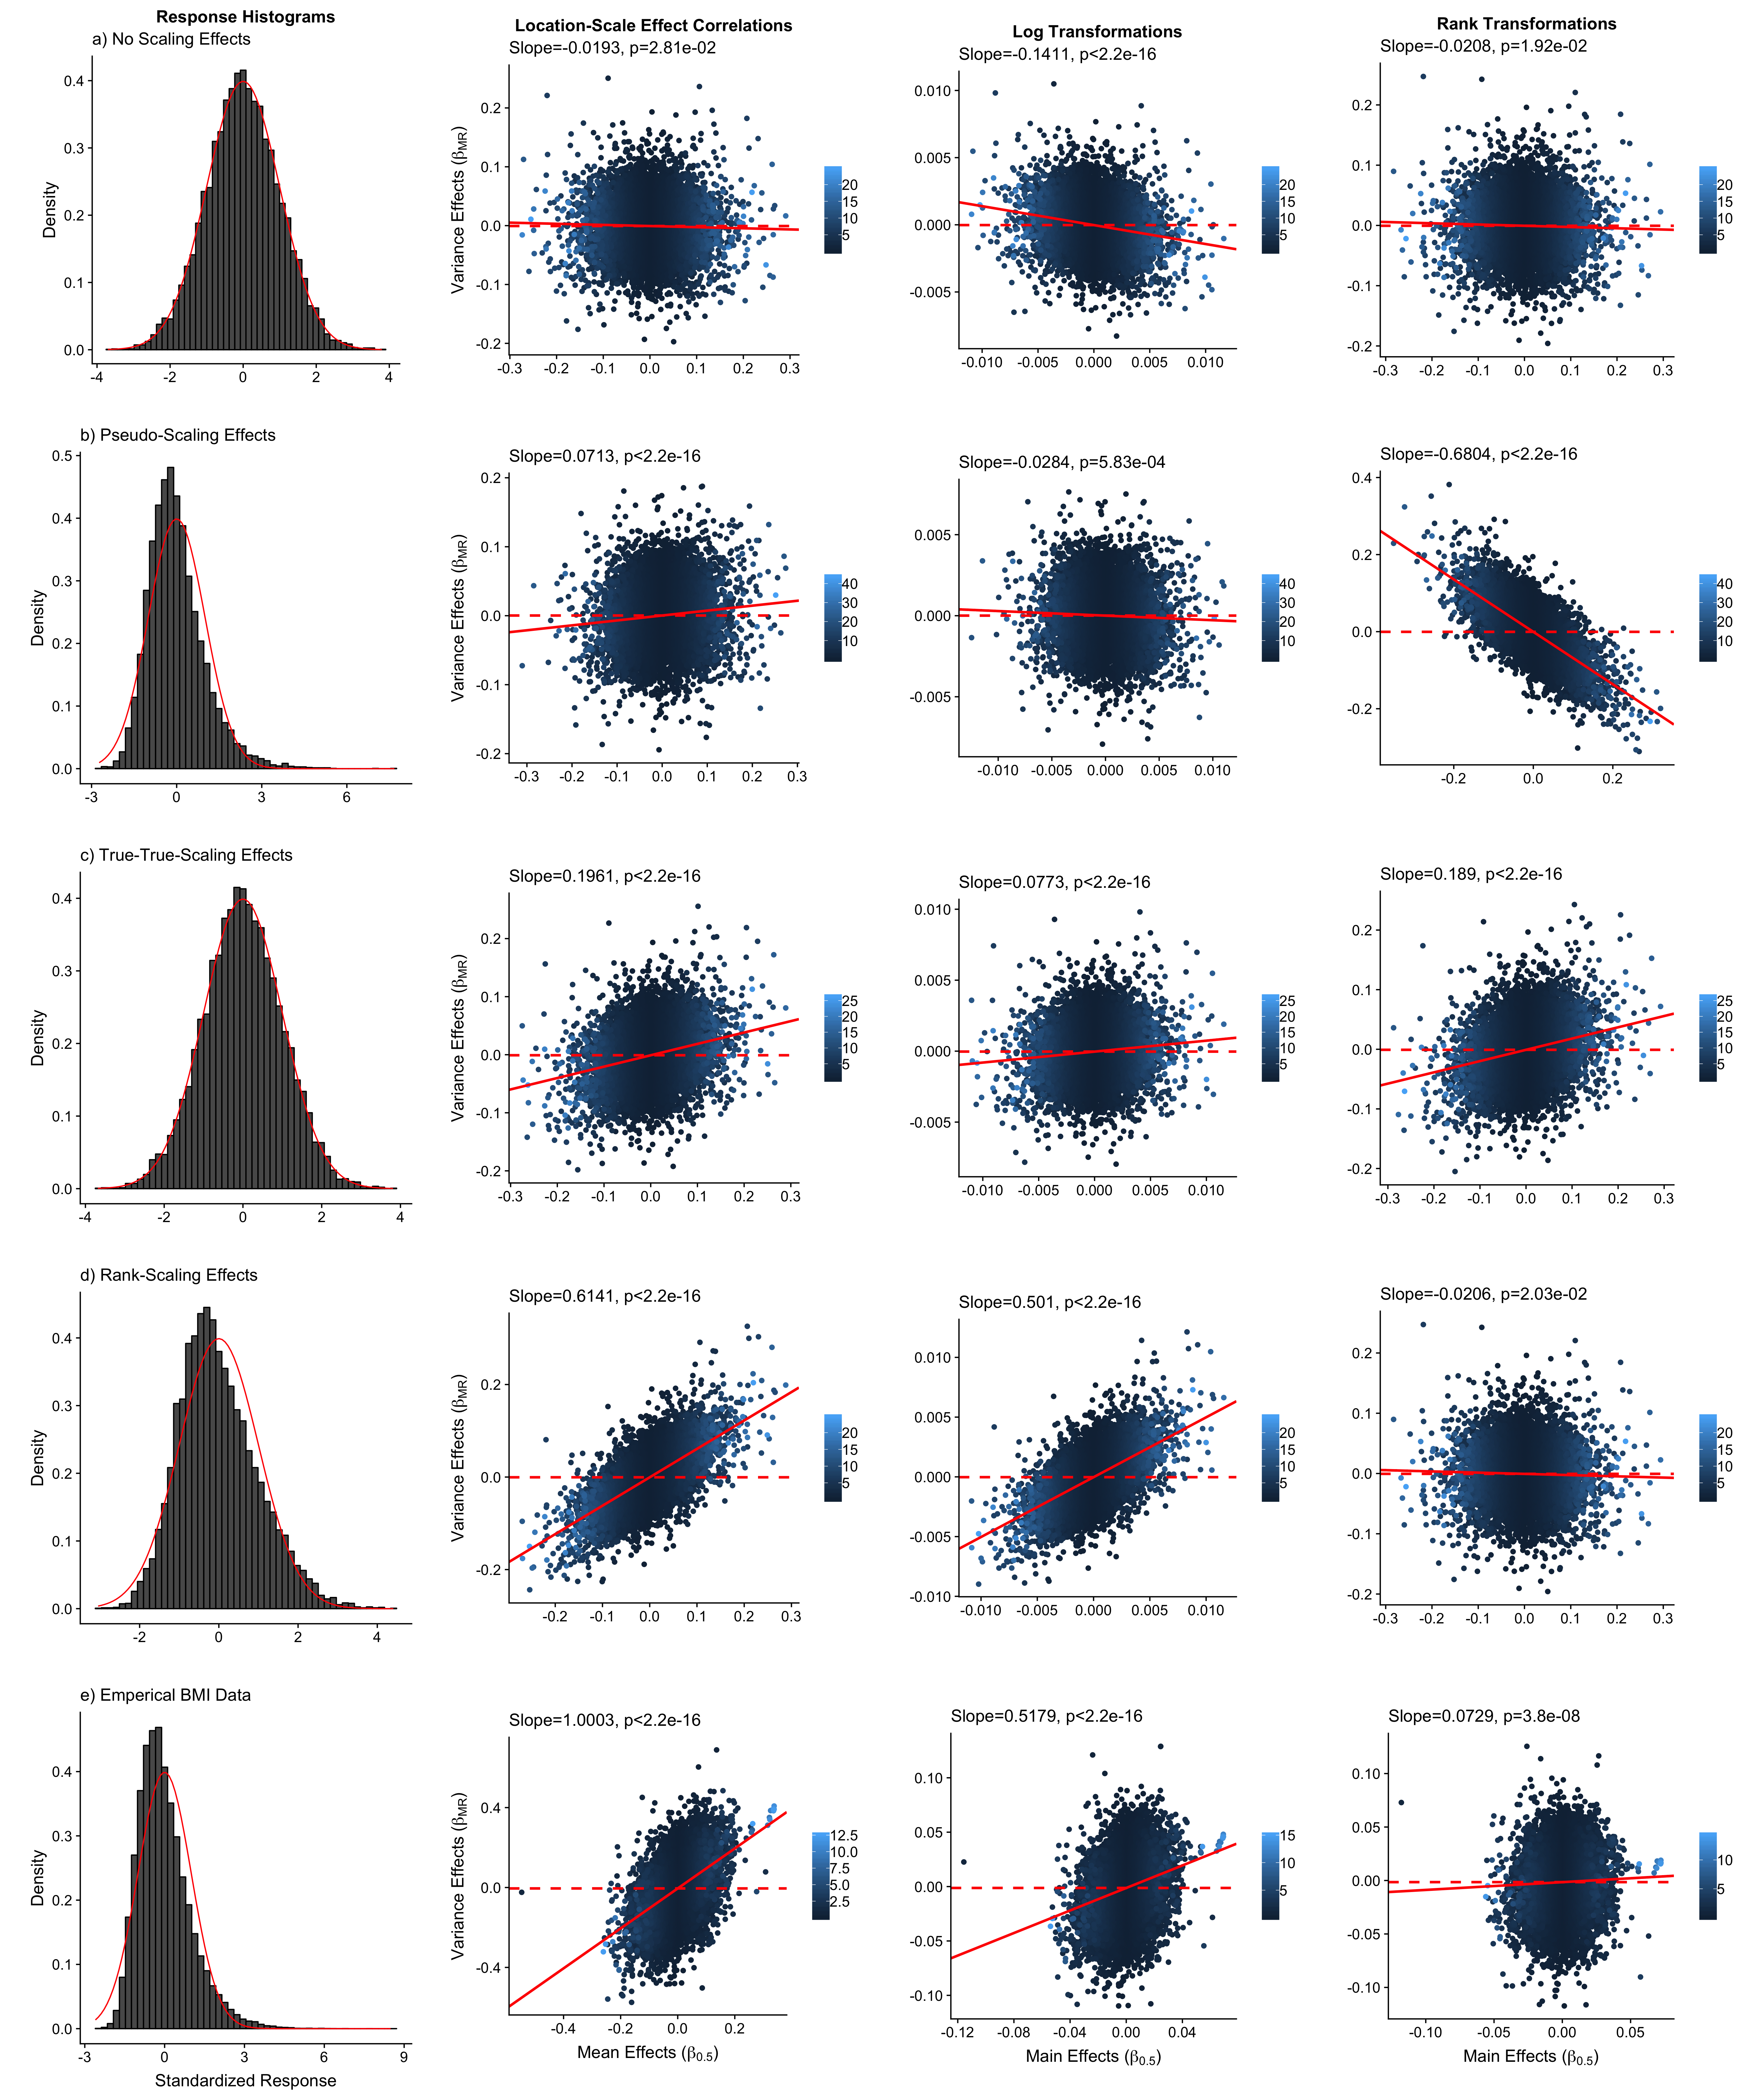
\includegraphics[width=1 \textwidth, height=1.2\textwidth]{Figures/Histograms_Scaling_Plots.png}
	\caption{Types of Scaling effects.}
	\label{fig:ScaleEffTypes}
\end{figure}

\newpage
	\begin{figure} 
	\centering
	\includegraphics[width=1 \textwidth, height=1.2\textwidth]{Figures/MQR_Manhattan_Plots.png}
	\caption{MQR Manhattan Plots.}
	\label{fig:ManhattanPlots}
\end{figure}

\newpage
\begin{landscape}
	\centering
	\begin{figure} 
		\centering
		\includegraphics[width=1 \textwidth, height=0.55\textwidth]{Figures/Table_1.pdf}
		\caption{Table 1: Empirical Results.}
		\label{fig:Table_1_EmpiricalResults}
	\end{figure}
\end{landscape}

\newpage
\begin{landscape}
	\centering
	\begin{figure}[h!]
		\centering
		\includegraphics[width=1 \textwidth, height=0.55\textwidth]{Figures/FP_R004_2.jpg}
		\caption{Type I error rates for test statistics of potential interactions. The error bars corresponds to the binomial confidence interval for $R=10,000$ replications. $R^{2}_G$ corresponds to the variance explained by the genetic variant's main effect. The variance explained by the interacting variable is fixed at $24\%$. The $G\times E$ test corresponds to the reference direct interaction using median CQR. Levene and BF correspond to the variance heterogeneity tests by Levene and the Brown-Forsythe F-tests respectively. Unadj-MUQR and MUQR corresponds to UQR models fitted on the raw and residuals scale of the response variable}
		\label{fig:FP}
	\end{figure}
\end{landscape}

\newpage
\begin{figure}[h!]
	\centering
	\includegraphics[width=1 \textwidth, height=0.6\textwidth]{Figures/power_nominal_cVar23_t.jpg}
	\caption{Power of detecting interaction effects for 2 and 3 genotype group levels}
	\label{fig:PowLevel}
\end{figure}

\newpage
\begin{figure}[h!]
	\centering
	\includegraphics[width=1 \textwidth, height=0.85\textwidth]{Figures//Power_Int.jpg}
	\caption{Power of detecting synergistic interaction effects. Power is presented for when the error distribution is symmetric ($\alpha_\epsilon = 0$) or asymmetric ($\alpha_\epsilon = 20$).  The interacting variable is simulated from a standard normal relevance variance explained fixed at $R^{2}_{X}=24\%$. MAF was fixed at $5\%$ as there are no to minor differences in power due to re-adjustment of interaction effects to keep $R_{G \times E}$ fixed as intended.}
	\label{fig:Pow1}
\end{figure}

\newpage
\begin{figure}[h!]
	\centering
	\includegraphics[width=0.6 \textwidth, height=0.6\textwidth]{Figures/Power_Curves_Scaling_Adjusted.png}
	\caption{Simulation results of Scaling effect adjustments}
	\label{fig:ScaleEffPower}
\end{figure}

\begin{figure}[h!]
	\centering
	\includegraphics[width=1.2\textwidth, height=1.2\textwidth]{Figures/Main_Variance_Effects_w_Scaling_Model.png}
	\caption{Summarizing main and variance effects of SNPs that passed the multiple testing correction threshold and including the scaling model}
	\label{fig:MainVarianceEffectsSelectSNPs}
\end{figure}

\begin{figure}[h!]
	\centering
	\includegraphics[width=1\textwidth, height=1\textwidth]{Figures/Interaction_vs_Scaling_Variance_Effects.png}
	\caption{Separating total variance effects into component that is attributed to scaling and component that is attributed to potential gene interactions.}
	\label{fig:Interaction_vs_ScalingEffectsSelectSNPs}
\end{figure}




\newpage
\begin{appendices}
\beginsupplement
\section{Supplementary Material}

\subsection{Model Formulations}
\indent \indent To formally introduce and illustrate the utility of QR in genome-wide association analysis, consider the response vector $Y$ from $n$ independent and identical distributed (i.i.d) samples with $cdf$ $F_{Y}\left(y\right)$. Assume the following linear model
\begin{equation} \label{mod1}
y_i = \beta_0 + \beta_1 x_i + \beta_2 g_i + \beta_3 x_i g_i + \epsilon_i
\end{equation}
where $x_i$ corresponds to an interacting variable with $X \sim F_X (\mu_x,\sigma_x^2)$; $g_i$ is the observed genotype of the genetic variant, $G$, under HWE with the population allele frequency, $p$, where $G \sim Bin(2, p)$; and $\epsilon_i$ is the random error with $\epsilon \sim F_{\epsilon} (0, \sigma_\epsilon)$. $\beta_0$, $\beta_1$, $\beta_2$ and $\beta_3$ correspond to the intercept, marginal effect of the interacting variable, marginal effect of the genotype, and the interaction effect between them, respectively. The conditional distribution of $Y$ can be described as $F_{Y \mid X=x,G=g} \sim \left(\beta_0 + \beta_1 x + \beta_2 g + \beta_3 xg, \sigma_y^2 \right)$. 
Assuming that $X$ and $G$ are independent, then the conditional density of $Y$ given $G$ can be shown to have a mean and variance: 
\begin{equation} 
\begin{split}
E \left[Y \mid G=g \right] &= (\beta_0 + \beta_1 \mu_x) + (\beta_2 + \beta_3 \mu_x)g 
%&= \beta_0^* + \beta_1^*g
\end{split}
\end{equation}
\begin{equation} \label{CondVar}
\begin{split}
Var(Y \mid G=g) = \sigma_x^2 (\beta_1 + \beta_3 g)^2 + \sigma_\epsilon^2
\end{split}
\end{equation}
Note that $c=\beta_1 + \beta_3 g$ is an amplification factor for the conditional variance that corresponds to the remaining variability in $Y$ given $G$. Under an additive genetic model, response variances by genotypes are all equal if and only if $\beta_3 =0$. Hence, tests of differences in response variance per genotype can identify variants with potential interactions \cite{pare2010use, gauderman2013finding}. Note that the conditional variance per genotype has a minimum at $\beta_3 = - \beta_1$. If the marginal and interaction effects are in opposite directions, then the power to detect potential interactions is reduced and therefore failure to identify differences in variance by genotype effects does not rule out interactions effects \cite{struchalin2010variance}. Equation \ref{CondVar} indicates that gene interactions will increase or decrease variance consistently across genotype levels. However, tests for variance heterogeneity detect variance inconsistency rather than variance structure (i.e. direction of change). Variance heterogeneity is not specific to interaction signals, but includes conditions where no consistent direction for increasing or decreasing variance per genotype are observed. Modeling the relationship between variance and genotype assuming a structure (i.e. a linear trend) could improve power to detect potential interactions. This can be done as a reformulation of the heteroscedasticity in equation \ref{CondVar} into a QR framework. The linear scale model of heteroscedasticity [i.e. $\sigma(x) = (1 + x\theta)\sigma$] is a special case of QR models with linear conditional quantile functions. Note that other models of systematic heteroscedasticity can be approximated for small $\theta$ by a linear expansion \cite{koenker1982robust}. This includes multiplicative heteroscedasticity in the form of $\sigma(x) = e^{x\theta}$ \cite{harvey1976estimating, godfrey1978testing}. Hence, assuming a linear heteroscedastic function is reasonable for variants with small interaction effects. Nonetheless, modest interaction effects require the correct heteroscedasticity function (i.e. linear, or nonlinear) to detect, while small interaction effects may remain difficult to identify and/or non-clinically relevant.  

To reformulate heteroscedasticity into the QR framework, let $\epsilon_x$ be the partial error for the unadjusted interacting variable $X$ with mean zero and variance $\sigma_x^2$. Then the conditional distribution $F_{Y \mid G}(y \mid G=g)$ can be translated into a heteroscedastic linear model with partitioned residuals where $\sigma_{\epsilon_{x}}(g) = (\beta_1 + \beta_3 g)$. That is 
\begin{equation} \label{hetMod}
\begin{split}
y_i &= \big(\beta_0+\beta_1 \mu_x\big) + \big(\beta_2 + \beta_3 \mu_x\big)g_i + \big(\beta_1 + \beta_3 g_i\big) \epsilon_{x,i} + \epsilon_{i} 
\end{split}
\end{equation}
%\\
%&=(\beta_0+\beta_1 + \beta_1 \epsilon_{i,1} + \epsilon_{i,2}) + (\beta_2 + \beta_3 \mu_x + \beta_3 \epsilon_{i,1})g_i 
The conditional quantile function for the heteroscedastic model under i.i.d errors is
% \sim F_{\epsilon_1}(0, \sigma_x^2)$, $\epsilon_2 \sim F_{\epsilon_2}(0, \sigma_\epsilon^2)$. 
\begin{equation} \label{firstQR}
\begin{split}
Q_Y (\tau \mid G=g) = \beta_0 (\tau) + \beta_G (\tau)g
\end{split}
\end{equation}
where
\begin{equation*} 
	\begin{split}
		\beta_0(\tau) &= \beta_0+Q_{\epsilon}(\tau)+\beta_1 \big[\mu_x+Q_{\epsilon_x}(\tau)\big] \\
		\beta_G (\tau) &= \beta_2 + \beta_3\big[\mu_x + Q_{\epsilon_x}(\tau)\big]
	\end{split}
\end{equation*}
Assuming that $X$ and $G$ are independent (i.e. $E\big[X \mid G=g\big]=E\big[X\big]$) for simplicity, the effects of genetic variant $G$ on the $\tau$-th quantile of $Y$ are equal (i.e. $\beta_G (\tau) = \beta_2$ for all $\tau \in (0,1)$) if and only if $\beta_3=0$. $\beta_G (\tau)$ is in fact a linear function of $Q_{\epsilon_x}(\tau)$ with slope given by interaction coefficient $\beta_3$. Overall, $\beta_G (\tau)$ inherits properties of $Q_{\epsilon_x}(\tau)$ that include monotonicity with $\tau$ and captures both variability, and skewness of the interacting variable $X$. An example is provided in the Supplementary Material.  

\subsection{Modeling QR Estimates}
\indent \indent Let the vector $\bm{\beta_G(\tau)}$ correspond to a vector of quantile estimates at $\bm{\tau}$ quantiles of the response. Modeling and testing the dependency structure of $\bm{\beta_G(\tau)}$ with $\bm{\tau}$ can be used as an overall robust indicator of potential interactions. Note that no parametric assumptions on partial errors due to interaction variables are required. Let $\bm{\widehat{\beta}}_G(\tau)$ and $\bm{\widehat{\Sigma}}_G$ denote the subset of QR regression estimates and the corresponding variance-covariance matrix. The relationship between genetic effects and percentiles $\boldsymbol{\tau}$ centered at the median can be investigated using MR (also known as generalized least squares).

Let $A= \begin{pmatrix} \bm{1}^{'} && \bm{\tau}^{*} \end{pmatrix}$ be the design matrix, where $\bm{\tau}^{*} = \bm{\tau} - 0.5$. The regression coefficients of MR models are given by
\begin{equation}
\begin{split}
\bm{\widehat{\beta}}_M &= \big(A^{t}\bm{\widehat{\Sigma}}_{G}^{-1} A \big) A^{t} \bm{\widehat{\Sigma}}_{G}^{-1}\bm{\widehat{\beta}}_{G}(\tau) \\
&=\begin{pmatrix} \widehat{\beta}_G && \widehat{\beta}_\tau \end{pmatrix}
\end{split}
\end{equation}
with variance-covariance matrix of the estimates 
\begin{equation*}
	\bm{\widehat{\Sigma}}_M=A^{t}\bm{\widehat{\Sigma}}_{G, \tau}^{-1} A
\end{equation*}
In this formulation, $\widehat{\beta}_G$ and $\widehat{\beta}_\tau$ correspond to the variant's estimated marginal and quantile-widening effects, respectively. The magnitude and direction of $\beta_\tau$ reflect quantiles of the partial error(s) density, $\bm{\epsilon_X}$, which vary according to interaction effects, marginal effects, and the variance-covariance matrix of interacting variables. \textcolor{red}{MOVE TO DISCUSSION The density of interacting variables is specific to sample population of interest, and one may consider that differences in $\beta_\tau$ between populations may reflect differences in the density of interacting variables (i.e. differences in exposures of different populations to interacting variables)}. For simplicity, the use of MR to estimate the variability of QR estimates by $\tau$ will henceforth be referred to as meta-quantile regression (MQR), meta-conditional quantile regression (MCQR), and meta-unconditional quantile regression (MUQR) as needed.

We provide an analytical description for how MQR captures these properties under the null hypothesis of no interactions (\textcolor{red}{Supplementary Material}). Moreover, CQR estimates have been shown to asymptotically converge to a normal distribution under i.i.d errors \cite{koenker1982robust, powell1984least, kim2003estimation}. These asymptotic properties of CQR estimates have varying convergence rates that weaken with extreme distribution tails \cite{chernozhukov2005extremal}. As a result, modeling extreme quantiles may require bootstrap methods to limit reliance on the assymptotic convergence of these estimates \cite{chernozhukov2016extremal}. Bootstrap methods provide the means to characterize the joint normal density of estimates across quantiles. Nonetheless, bootstrap methods can be computationally intensive for large models and samples as in classic GWAS study designs. To our knowledge, there are no studies assessing the asymptotic convergence rate of $\widehat{\beta} (\tau)$ and $\widehat{\Sigma}_G$ from UQR models. Note that $\widehat{\Sigma}_G$ from UQR models using least-squares regression is the variance-covariance matrix of multivariate regression errors given as $\vfrac{\bm{\epsilon^{'}} \bm{\epsilon}}{(n-r-1)}$, where $r$ is the number of predictors. Provided that $\Sigma_M$ was estimated correctly, a linear trend with $\bm{\tau}$ can be tested using $H_0: \beta_{\tau}=0$ as,
\begin{equation}
Z_{\tau}=\frac{\widehat{\beta}_{\tau}}{SE_{\widehat{\beta}_{\tau}}} \sim N(0,1)
\end{equation}
The process of computing $Z_\tau$ for UQR is different from CQR. UQR requires adjustment for the main effect of genotypes where $Z_\tau$ is computed on residuals of $Y$ regressed against $G$. To explain why, consider the earlier example in equation \ref{firstQR} and the special case where $\beta_0=\beta_1=0$, $\beta_2\neq 0$ and $\beta_3\neq 0$. The implication of the heteroscedasticity function $\sigma_x (g) = \beta_3 g$ on the conditional quantile function of $Y$ is
\begin{equation}
\begin{split}
\textrm{Pr}\big[Y>q_\tau\mid G=g\big] &= \textrm{Pr}\big[g(\beta_2+\beta_3 \epsilon_x)+ \epsilon) > q_\tau\big] \\
&=\textrm{Pr}\big[\epsilon_x > \frac{q_\tau - \beta_2 g - \epsilon}{\beta_3 g}\big] \\
&= 1-F_{\epsilon_x} \big(\frac{q_\tau - \beta_2 g - \epsilon}{\beta_3 g}\big) 
\end{split}
\end{equation}
where a change in $G$ corresponds to a change in both the numerator and denominator given the directions and magnitudes of $\beta_2$ and $\beta_3$. The presence of both marginal and interaction effects complicates the relationship between genotypes and the `unconditional' quantiles of $Y$ that UQR models. UQR utilizes observed sample quantiles as approximations to the unobserved unconditional quantiles of $Y$ for re-centered influence function (RIF) transformations at a given vector of percentiles, $\bm{\tau}$. This is problematic because sample quantiles are `contaminated' by $g$ where the mixture of marginal and interaction effects compromise trends in $\bm{\beta_G (\tau)}$ with $\bm{\tau}$ (See Supplementary). This can be overcome using the residuals of the response adjusted for genotype effect. The marginal effect of $g$ is treated as a nuisance parameter using a two-step estimation approach through modeling quantiles of $Y^* = Y - g\widehat{\beta}(\tau=0.5)$, where $\widehat{\beta}(\tau=0.5)$ is the marginal effect estimated using UQR. Note that CQR models the conditional quantile function of $Y$, and hence, do not suffer from this limitation of UQR. 

Choosing the appropriate number and range of percentiles to consider for CQR and UQR depend on the sample size given that our framework assumes that QR estimates converge to the true population estimates and are normally distributed. Supplementary Supplementary Figure ~\ref{fig:FS1} \textcolor{red}{need to redo these figures for CQR with bootsrap} shows the convergence of $Z_{\tau}$ from CQR and UQR estimates toward nominal Type I error rate of $0.05$. Deviations from the null distribution mainly occur when modeling extreme quantiles and, to a lesser extent, by the number of quantiles modeled. Nonetheless, hypothesis tests for $Z_{\tau}$ using UQR estimates converge much faster to the correct null distribution compared to CQR estimates. 

\subsection{Modeling Scaling Effects}
\indent \indent We describe several conditions that induce correlations between estimates of marginal and quantile-widening effects, commonly known as scaling phenomena. 1) Scaling due to skewness, termed 'pseudo-scale effects'; 2) scaling due to linear heteroscedasticity as a function of marginal effects, termed 'true-scale effects'; and 3) rank-based scale effects. These three types of coerced correlations encompass the challenges of investigating  quantile-widening effects for variables with marginal effects on the response. We present a robust approach to adjust for such scaling effects so that quantile-widening effects can be ascribed to potential gene interactions. 

Pseudo-scale effects can arise when estimating marginal and quantile-widening effects on asymmetric outcome distributions. This can can be modelled using errors from skewed distributions, such as the skew-normal or exponential distribution. This type of scaling effect is analogous to the correlation between location and scale parameters of asymetric distributions. Here, marginal effects and quantile-widening effects are a function of a common skewness parameter (See Motivational Example in the Supplementary Materials) and the scaling effect is proportional to the degree of skewness. True-scale effects were defined as variance effects as a function of mean effects. Given a simple linear model with a heteroscedasticity function $(1+\gamma\beta_2)$, the conditional mean mean remains unchanged, but the conditional variance of $Y$ can be shown to be
\begin{equation} \label{TrueScaleMod}
Var(Y|G=g)=\sigma_x^2 (\beta_1+\beta_3 g)^2 + \sigma_\epsilon^2 (1+\gamma\beta_2 g)^2
\end{equation}
where $\gamma$ is the true scaling effect parameter due to genotype marginal effects $\beta_2$. This type of scaling effect can occur in symmetric and asymmetric distributions. \textcolor{red}{consider moving : True-scale effects can be reduced, but not eliminated, by log transformations and are unaffected by rank-based inverse normal transformations.} 

Lastly, to formulate a rank-based scale effect that can be treated by rank-based inverse-normal transformation, the outcome distribution for sample $y_i$  was linearly amplified by $\gamma (\tau, \omega)$ according to its rank, such that $\gamma (\tau, \omega) = 1 + \tau \omega$, where $\tau$ is the percentile rank, and $\omega$ is the rank-multiplier. Hence, the rank-conditional distribution for sample $y_i$ has mean and variance that are multiplicatively amplified by $\gamma (\tau, \omega)$. The derivations of mean and variance of the outcome distribution is not trivial in the context of non-i.i.d samples. The advantage of this method is that all terms with marginal effects, also have variance and quantile-widening effects because marginal effects shift sample ranks. Furthermore, the rank-multiplier induces a skewness in the outcome distribution that is treatable by inverse-normal rank-transformation which eliminates the effect of the rank-multiplier, $\omega$.  These three types of scaling are illustrated in ~\ref{fig:ScaleEffTypes}. It is evident that pseudo-scaling effects (row b) are relatively weak even with highly skewed distributions, while rank-scaling effects (row d) result in a strong correlation between marginal effects and quantile-widening effects relative to the degree of skewness. Rank-based inverse normal transformation exacerbates pseudo-scaling but eliminates rank-scaling. True-scaling (row c) does not result in any skewness, is reduced by log-transformation, and is unchanged by rank-based inverse normal transformations. \textcolor{red}{consider moving : Finally, we observed that the scaling effects of the BMI sample population (row e) appears stronger than expected for skewness alone and that some component of the scaling effect is rank-based as rank-based inverse normal transformation counteracts most, but not all, of the scaling effect.} 

Since scaling effects denote a proportionality between marginal and quantile-widening effects, it is reasonable to model this relationship using a regression approach. The goal is to decompose quantile-widening effects that are attributed to marginal effects (i.e. scaling) from quantile-widening effects that are attributed to potential interactions. This approach is flexible and supports linear/non-linear, additive/non-additive relationships. For simplicity, we assume additive linear scale effects and model scaling using robust regression (median regression) weighted by the \textcolor{red}{double check this : inverse-variance of marginal effects}. This scaling model can then be used to predict the quantile-widening effects from the marginal effects of SNPs (i.e. the quantile-widening effects predicted by scaling alone). The estimated quantile-widening effects of each SNP can then be adjusted using the scaling model according to their marginal effects. The scaling-adjusted quantile-widening effect and corresponding standard errors are given by
\begin{equation}
\begin{split}
\hat{\beta}_{MR_{adj}}&=\hat{\beta}_{MR} - \hat{\beta}_{SM} \\
s.e(\hat{\beta}_{MR_{adj}}) &= \sqrt{s.e(\hat{\beta}_MR)^2 + s.e(\hat{\beta}_{SM})^2}
\end{split}
\end{equation}
where $\hat{\beta}_{SM}$ is the predicted variance effect given mean effects.


\subsection{The differences between CQR and UQR}

\indent \indent The terms ``conditional'' and ``unconditional'' refer to the type of quantiles modeled by each of the two methods. CQR models quantiles of the response variable in the form of a conditional distribution (i.e. $Q_{Y \mid X_1, X_2}(\tau \mid X_1=x_1, X_2=x_2)$, where $X_1$ and $X_2$ are two explanatory variables). The coefficients of explanatory variables in CQR models are conditional effects. They are average effects on population quantiles given information on all other explanatory variables. There is a growing consensus in the literature that many researchers have misused CQR by misinterpreting coefficients \cite{killewald2014motherhood}. Unfortunately, the law of iterative expectations do not apply for conditional quantile functions. Hence, integrating out other conditioning explanatory variables is necessary to obtain an interpretable marginal effect. However, the difficulty shifts from coefficient interpretations to integration methods that may not work (i.e. sparse data) and their computational overheads. Examples of integration approaches are provided by Melly B. and Powell D. \cite{powell2016quantile, melly2015changes}. The marginalization of CQR coefficients remains an active research area \cite{angrist2008mostly, gushchin2018integrated}. Other methods for marginalizing quantile regression estimates include UQR that was introduced by Fripo 2009 \cite{firpo2009unconditional}. UQR is based on the concept of re-centered influence functions (RIF) that transform the response into a new variable having asymptotic mean and variance statistics equal to that of the sample quantile. Hence, the transformed variable can be modeled as a function of explanatory variables using OLS regression where coefficients are interpreted as marginal effects (i.e. $E\big[RIF(Y, \tau) \mid X_1=x_1, X_2=x_2 \big] = \beta_0 + \beta_1 x_1 + \beta_2 x_2$) \cite{firpo2009unconditional}. In short, UQR approximates and models unconditional quantile of the response variable post removal of 'contamination' by the explanatory variables \cite{firpo2009unconditional}. It is straightforward and is computationally inexpensive given closed form solutions. 

Overall, both CQR and UQR models provide similar unadjusted estimates using univariable models where both estimates are marginal effects. This is because CQR estimates are not conditioned on other explanatory variables that need to be integrated out. The difference between CQR and UQR lies in adjusted estimates using multvariable regression models with two or more explanatory variables. 

\subsection{Motivational Example}
Quantile regression estimates of genetic variants across the sample distribution capture the location, scale, and shape of interacting variables. To show this, let's consider simulating the interacting variable, $X$, from a skew-normal distribution, $SN(\zeta, \omega, \alpha)$, with location ($\zeta$), scale ($\omega$), and shape ($\alpha$) parameters. The mean and variance of $X$ are given as 
\begin{equation} \label{SNpars}
\begin{split} 
\mu_x &= \zeta + \omega\delta \sqrt{\vfrac{2}{\pi}} \\
\sigma_x^2 &= \omega^2 \big(1-\vfrac{2 \delta^2}{\pi}\big)
\end{split}
\end{equation}
where 
\begin{equation}
\delta = \vfrac{\alpha}{\sqrt{1+\alpha^2}}
\end{equation} 

The partial residual, $\epsilon_x$, follows the same distribution family of $X$ but with a mean of zero. That is, a skew-normal distribution with a location parameter, $\zeta=-\omega \delta \sqrt{\vfrac{2}{\pi}}$, such that $\mu_{\epsilon_x} =0$. We simulated independent and identically distributed (i.i.d.) samples from $X$, and $G$, with error $\epsilon$. The response , $Y$, is generated as given in equation \ref{mod1} with coefficients $\beta_1=1$, $\beta_2=0$, $\beta_3=1, 0$, or $-1$ under different scale and shape parameters for the interacting variable $X$. Interaction effects with the same direction as the marginal effects are called synergistic interaction effects (e.g. $\beta_1=1$ and $\beta_3=1$), where as interactions with opposite direction of effects are called antagonistic interaction effects (e.g. $\beta_1=1$ and $\beta_3=-1$). The sample size was set to $n=10000$. $G$ and $\epsilon$ are simulated from a binomial with minor allele frequency ($MAF$) of $0.5$ and a standard normal distribution, respectively. Lastly, CQR and UQR were fitted and compared to the truth given in equation \ref{firstQR}. Note that CQR and UQR produce similar estimates for univeriable models (Supplementary Material). Figure \ref{fig:MotExample} shows CQR and UQR estimates under an unadjusted interacting variable $X$ with different scale and shape parameters. An increase in the scale parameter of $X$ results in a larger slope of $\beta(\tau)$ with $\tau$, while the increasing the skewness shifts $\beta(\tau)$ vertically corresponding to the direction of the interaction effect as $\omega\delta \sqrt{\vfrac{2}{\pi}}$. Note that in the case of perfect antagonistic interactions where $\beta_1=-\beta_3$, the resulting QR estimates correspond to a shift in interacting variable ($\omega\delta \sqrt{\vfrac{2}{\pi}}$). This can be easily seen if we consider the effect of such interactions on the heterosdastic model in equation \ref{hetMod} where $y_i$ becomes $\big(\beta_0+\beta_1 \mu_x\big) + \big(\beta_2 + \beta_3 \mu_x\big)g_i + \epsilon_{i}$. Hence, QR curves characterize the distribution of interacting variables(s), where we note that skewness results in vertical shifts similar to marginal effects. 

\begin{figure}[h!]
	\centering
	\includegraphics[width=0.75 \textwidth, height=1.25\textwidth]{Figures/QR_EXAMPLE_July148.jpg}
	\caption{Genetic effects across percentiles for interacting variables with different scale and shape parameters.}
	\label{fig:MotExample}
\end{figure}

\newpage
\begin{figure}[!h]
	\centering
	\includegraphics[width=1\textwidth, height=0.8\textwidth]{Figures/CQRvsUQR_Speed.jpg}
	\caption{Computational Efficiency of UQR over CQR. The computational time for UQR scales well with all number of snps, sample size, percentiles, and covariates compared to CQR. CPU time for UQR included time required for RIF transformation.}
	\label{fig:CompEff}
\end{figure}

\newpage
\begin{landscape}
	\begin{figure}%[h!]
		\centering
		\includegraphics[width=1\textwidth, height=0.5\textwidth]{Figures/ConvergenceDiag_Rate.jpg}
		\caption{Type I error rate for the number and range of percentiles by sample size. UQR estimates (blue) are more asymptoticly efficient than CQR estimates (red)} 
		\label{fig:FS1}
	\end{figure}
\end{landscape}
%\includepdf{ConvergenceDiag_Rate.jpg}
% , , angle=90

\newpage
\begin{figure}[h!]
	\centering
	\includegraphics[width=0.8 \textwidth, height=0.45\textwidth]{Figures/power_nominal_cVar45.jpg}
	\caption{Power of detecting interaction effects for 4 and 5 genotype group levels.}
	\label{fig:PowLevel45}
\end{figure}

\newpage
\subsection{Multiple Interactions}
\indent \indent The formulation of heteroscedasticity due to unadjusted interactions as given in equation \ref{firstQR} can be generalized further for a set of $k$ independent interacting variables in matrix form as
\begin{equation}
\begin{split}
Q_Y (\tau \mid G=g) = A \beta (\tau)
\end{split}
\end{equation}
where $A$ is the design matrix $\begin{pmatrix} \bm{1} & G^{'} \end{pmatrix}$ and 
\begin{equation}
\begin{split}
\beta (\tau)=    
\begin{pmatrix}
\beta_0+ \sum_{j=1}^{k} \beta_{x_j}\mu_{x_j} \\
\beta_g + \sum_{j=1}^{k}\beta_{int_j}\mu_{x_j} 
\end{pmatrix} +
\begin{pmatrix}
\sum_{j=1}^{k} \beta_{x_j} Q_{\epsilon_{j}}(\tau) + Q_{\epsilon_{k+1}}(\tau) \\
\sum_{j=1}^{k} \beta_{int_j} Q_{\epsilon_{j}} (\tau) 
\end{pmatrix}
\end{split}
\end{equation}
Here, $\beta_g$ and $\beta_{x_{j}}$ are the marginal effects of the genetic variant and $k$ interacting variables, while $\beta_{int_j}$ are their respective interaction coefficients. The cumulative two-way interactions of $k$ variables results in a linear heteroscedastic function $\bm{1}^{'}\bm{\gamma}$ where $\gamma$ has elements $\sigma_j(g) = \beta_{x_j} +  \beta_{int_j} g$. 
%The main effect of the genetic variant $\beta_g$ is a fixed constant for all $\bm{\tau} \in \tau_1,...,\tau_m$ if and only if all interacting effects, $\beta_{int_j} = 0$. 

We can further break down the independence assumption between interacting variables given a joint CDF $F_{\bm{X}}$ with their corresponding mean vector and variance-covariance matrix $\bm{\Sigma_X}$. The multivariate density of their corresponding errors $\bm{\epsilon_X}$, $F_{\bm{\epsilon_X}}$, captures the same shape and scale of $F_{\bm{X}}$ with a mean vector of zero and variance-covariance matrix $\bm{\Sigma_X}$. In this case, $\beta_G (\tau)$ changes with the multivariate quantile function $Q_{\bm{\epsilon_X}}$ \cite{chaudhuri1996geometric}. This formulation highlights that QR estimates of $\beta_G (\tau)$ represent contour lines at $\bm{\tau}$ given the joint density of $k$ interacting variables weighted by degree of interaction effects. In this regard, the modeling of QR estimates across phenotype distributions can be useful for identifying variants with potential interactions.

\subsection{Meta-regression of QR Estimates Under no Interactions }
\indent \indent This section aims to compute the MR parameter estimates to verify how the compares with the original linear model of two-way interactions given in equation \ref{mod1}. Let's define $A$ and $\Sigma_G$ as the design matrix and the cross-distribution variance-covariance matrix for $\beta_G (\tau)$ estimates. The closed solution for MR coefficients are given as:
\begin{equation}
\begin{split}
\bm{\widehat{\beta}}_M &= \big(A^{'}\bm{\Sigma}_G^{-1} A \big) A^{'} \bm{ \Sigma}_G^{-1}\bm{\beta_G(\tau)} \\
&=\begin{pmatrix} \widehat{\beta}_G && \widehat{\beta}_\tau \end{pmatrix}
\end{split}
\end{equation}
where $\widehat{\beta}_G$ and $ \widehat{\beta}_\tau$ correspond to the variant's marginal and slope for percentiles respectively. Under the null hypothesis of no interactions($H_0: \beta_3 =0$), 
$\beta_G (\tau)^{'} = \begin{pmatrix} \beta_g & \cdots & \beta_g \end{pmatrix}$. The design matrix of MR, $A$ is given by 

\begin{equation}
\begin{split}
A =  
\begin{pmatrix}
1 & \tau_1 \\
\vdots & \vdots \\
1 & \tau_m
\end{pmatrix}
\end{split}
\end{equation}
Let's further denote the inverse matrix of $\Sigma_G$ as 
\begin{equation}
\begin{split}
\Sigma^{-1}=   
\begin{pmatrix}
w_{11} &  \cdots & w_{1m} \\
\vdots & \ddots & \vdots \\
w_{m1} &  \cdots & w_{mm}
\end{pmatrix}
\end{split}
\end{equation}
The initial matrix computations as parts can be given as: 
\begin{equation}
\begin{split}
A^{'}\Sigma^{-1}A &=   
\begin{pmatrix}
\sum_{i=1}^{m}w_{i1} &  \cdots & \sum_{i=1}^{mm}w_{im} \\
\vdots & \ddots & \vdots \\
\sum_{i=1}^{m} \tau_i w_{i1} &  \cdots & \sum_{i=1}^{mm} \tau_i w_{im}
\end{pmatrix}  
\begin{pmatrix}
1 &   \tau_1 \\
\vdots  & \vdots \\
1 &   \tau_m
\end{pmatrix} \\ &= 
\begin{pmatrix}
\sum_{i=1}^{m} \sum_{j=1}^{m} w_{ij} &   \sum_{i=1}^{m} \tau_i \sum_{j=1}^{m} w_{ij} \\
\sum_{i=1}^{m} \sum_{j=1}^{m} \tau_i w_{ij}  & \sum_{i=1}^{m}  \tau_i \sum_{j=1}^{m} \tau_i w_{ij} 
\end{pmatrix}  
\end{split}
\end{equation}
Note that 
\begin{equation}
\begin{split}
(A^{'}\Sigma^{-1}A)^{-1} &= \frac{1}{C}  
\begin{pmatrix}
\sum_{i=1}^{m}  \tau_i \sum_{j=1}^{m} \tau_i w_{ij} & - \sum_{i=1}^{m} \tau_i \sum_{j=1}^{m} w_{ij}\\
-\sum_{i=1}^{m} \sum_{j=1}^{m} \tau_i w_{ij} & \sum_{i=1}^{m} \sum_{j=1}^{m} w_{ij}
\end{pmatrix} 
\end{split}
\end{equation}
where $C = \big(\sum_{i=1}^{m} \sum_{j=1}^{m} w_{ij}\big) \big(\sum_{i=1}^{m}  \tau_i \sum_{j=1}^{m} \tau_i w_{ij}\big) - \big( \sum_{i=1}^{m} \tau_i \sum_{j=1}^{m} w_{ij}\big) \big(\sum_{i=1}^{m} \sum_{j=1}^{m} \tau_i w_{ij} \big)$

Furthermore, 
\begin{equation}
\begin{split}
A^{'}\Sigma^{-1}A \beta(\tau) &=   
\begin{pmatrix}
\sum_{i=1}^{m}w_{i1} &  \cdots & \sum_{i=1}^{mm}w_{im} \\
\vdots & \ddots & \vdots \\
\sum_{i=1}^{m} \tau_i w_{i1} &  \cdots & \sum_{i=1}^{mm} \tau_i w_{im}
\end{pmatrix} 
\begin{pmatrix}
\beta_g \\ \vdots \\ \beta_g 
\end{pmatrix} \\ &= 
\begin{pmatrix}
\beta_g \sum_{i=1}^{m} \sum_{j=1}^{m} w_{ij} \\ 
\beta_g \sum_{i=1}^{m} \sum_{j=1}^{m} \tau_i w_{ij} 
\end{pmatrix}
\end{split}
\end{equation}

Hence,
\begin{equation}
\begin{split}
\widehat{\beta}_M &= (A^{'}\Sigma^{-1}A)^{-1} A^{'}\Sigma^{-1}A \beta(\tau) \\ &= \frac{1}{C}
\begin{pmatrix}
\sum_{i=1}^{m}  \tau_i \sum_{j=1}^{m} \tau_i w_{ij} & - \sum_{i=1}^{m} \tau_i \sum_{j=1}^{m} w_{ij}\\
-\sum_{i=1}^{m} \sum_{j=1}^{m} \tau_i w_{ij} & \sum_{i=1}^{m} \sum_{j=1}^{m} w_{ij}
\end{pmatrix} 
\begin{pmatrix}
\beta_g \sum_{i=1}^{m} \sum_{j=1}^{m} w_{ij} \\ 
\beta_g \sum_{i=1}^{m} \sum_{j=1}^{m} \tau_i w_{ij} 
\end{pmatrix} \\&=
\frac{1}{C} \begin{pmatrix}
\beta_g \big[\big(\big(\sum_{i=1}^{m} \sum_{j=1}^{m} w_{ij}\big) \big(\sum_{i=1}^{m}  \tau_i \sum_{j=1}^{m} \tau_i w_{ij}\big) - \big( \sum_{i=1}^{m} \tau_i \sum_{j=1}^{m} w_{ij}\big) \big(\sum_{i=1}^{m} \sum_{j=1}^{m} \tau_i w_{ij} \big)\big] \\
\beta_g \big[
- \big(\sum_{i=1}^{m} \sum_{j=1}^{m} \tau_i w_{ij} \big)
\big( \sum_{i=1}^{m} \sum_{j=1}^{m} w_{ij}\big) + 
\big( \sum_{i=1}^{m} \sum_{j=1}^{m} w_{ij}\big) 
\big(\sum_{i=1}^{m} \sum_{j=1}^{m} \tau_i w_{ij} \big) \big]  \\ \end{pmatrix} \\ &= \frac{1}{C} \begin{pmatrix} \beta_g C \\ 0  \end{pmatrix} \\ &=  \begin{pmatrix} \beta_g \\ 0  \end{pmatrix}
\end{split}
\end{equation}
\end{appendices}

\subsection{Supplemental Acknowledgements}
\textbf{ARIC (phs000280.v3.p1):} The Atherosclerosis Risk in Communities Study is carried out as a collaborative study supported by National Heart, Lung, and Blood Institute contracts (HHSN268201100005C, HHSN268201100006C, HHSN268201100007C, HHSN268201100008C, HHSN268201100009C, HHSN268201100010C, HHSN268201100011C, \\and HHSN268201100012C). Funding for CARe genotyping was provided by NHLBI Contract N01-HC-65226. Funding for GENEVA was provided by National Human Genome Research Institute grant U01HG004402 (E. Boerwinkle). Individual-participant phenotypic and genotypic data was extracted from the following dbGaP datasets (phs000280.v3.p1, pht004062.v1.p1, pht004063.v1.p1, pht004064.v1.p1, pht004065.v1.p1, pht004032.v1.p1, \\pht004033.v1.p1, pht004034.v1.p1, pht004035.v1.p1, pht003266.v1.p1, pht000114.v2.p1, \\phg000079.v1). The authors would like to thank the participants, investigators and staff of the ARIC study for their important contributions.

\textbf{CARDIA (phs000285.v3.p2):} The Coronary Artery Risk Development in Young Adults Study (CARDIA) is conducted and supported by the National Heart, Lung, and Blood Institute (NHLBI) in collaboration with the University of Alabama at Birmingham (N01-HC95095 and N01-HC48047), University of Minnesota (N01-HC48048), Northwestern University (N01-HC48049), and Kaiser Foundation Research Institute (N01-HC48050). This manuscript was not approved by CARDIA. The opinions and conclusions contained in this publication are solely those of the authors, and are not endorsed by CARDIA or the NHLBI and should not be assumed to reflect the opinions or conclusions of either. Funding for CARe genotyping was provided by NHLBI Contract N01-HC-65226. Individual-participant phenotypic and genotypic data was extracted from the following dbGaP datasets (phs000285.v3.p2, pht001583.v2.p2, pht001632.v2.p2, pht001671.v2.p2, pht001720.v2.p2, pht001785.v2.p2, \\pht001857.v2.p2, pht001589.v2.p2, pht001645.v2.p2, pht001697.v2.p2, pht001744.v2.p2, \\pht001804.v2.p2, pht001851.v2.p2, pht001557.v2.p2, pht001737.v2.p2, pht001799.v2.p2, pht001845.v2.p2, pht001569.v2.p2, pht001601.v2.p2, pht001656.v2.p2, pht001715.v2.p2, pht001761.v2.p2, pht001811.v2.p2, pht001555.v3.p2, phg000091.v2.p1, phg000092.v2.p1). The authors would like to thank the participants, investigators and staff of the CARDIA study for their important contributions.

\textbf{CHS (phs000287.v5.p1):} The research reported in this article was supported by contract numbers N01-HC-85079, N01-HC-85080, N01-HC-85081, N01-HC-85082, N01-HC-85083, N01-HC-85084, N01-HC-85085, N01-HC-85086, N01-HC-35129, N01 HC-15103, N01 HC-55222, N01-HC-75150, N01-HC-45133, N01-HC-85239 and HHSN268201200036C; grant numbers U01 HL080295 from the National Heart, Lung, and Blood Institute and R01 AG-023629 from the National Institute on Aging, with additional contribution from the National Institute of Neurological Disorders and Stroke. A full list of principal CHS investigators and institutions can be found at http://www.chs-nhlbi.org/pi.html. This manuscript was not prepared in collaboration with CHS investigators and does not necessarily reflect the opinions or views of CHS, or the NHLBI. Support for the genotyping through the CARe Study was provided by NHLBI Contract N01-HC-65226. Individual-participant phenotypic and genotypic data was extracted from the following dbGaP datasets (phs000287.v5.p1, pht001452.v1.p1, pht001488.v1.p1, pht001489.v1.p1, pht001490.v1.p1, pht001491.v2.p1, pht001492.v1.p1, pht001493.v1.p1, pht001494.v1.p1, pht001495.v1.p1, pht001474.v1.p1, pht001475.v1.p1, phg000077.v1). The authors would like to thank the participants, investigators and staff of the CHS for their important contributions.

\textbf{Framingham (phs000007.v28.p1):} The Framingham Heart Study is conducted and supported by the National Heart, Lung, and Blood Institute (NHLBI) in collaboration with Boston University (Contract No. N01-HC-25195 and HHSN268201500001I). This manuscript was not prepared in collaboration with investigators of the Framingham Heart Study and does not necessarily reflect the opinions or views of the Framingham Heart Study, Boston University, or NHLBI. Funding for CARe genotyping was provided by NHLBI Contract N01-HC-65226. Funding support for the Framingham Metabolomics - Risk Factor Study: Gas Chromatography/Mass Spec - BMI/Lipids/Gluc dataset was provided by FHS contract supplement, NHLBI Intramural Funding. Funding support for the Framingham Central Metabolomics - HILIC - Installment 1 dataset was provided by NIH grant R01DK081572. Funding support for the Framingham Central Metabolomics - HILIC - Installment 2 dataset was provided by NIH grant R01 DK081572. Funding support for the Framingham Metabolomics (HILIC - Installment 1) dataset was provided by NIH grant R01 DK081572. Funding support for the Framingham Metabolomics (HILIC - Installment 2) dataset was provided by NIH grant R01 DK081572. Funding support for the Framingham Metabolomics (Hilic - installment 3) dataset was provided by NIH grant R01 DK081572. Individual-participant phenotypic and genotypic data was extracted from the following dbGaP datasets (phs000007.v28.p1, pht000009.v2.p10, pht000010.v3.p10, pht000011.v3.p10, pht000012.v3.p10, pht000013.v3.p10, pht000014.v3.p10, pht000015.v3.p10, pht000016.v3.p10, pht000017.v3.p10, pht000018.v4.p10, pht000019.v3.p10, pht000020.v3.p10, pht000021.v3.p10, pht000022.v4.p10, pht000023.v4.p10, pht000024.v4.p10, pht000025.v4.p10, pht000026.v3.p10, pht000027.v3.p10, pht000028.v3.p10, pht000029.v3.p10, pht000040.v4.p10, pht003099.v4.p10, pht000030.v7.p10, pht000031.v7.p10, pht000032.v6.p10, pht000033.v8.p10, pht000034.v7.p10, pht000035.v8.p10, pht000036.v8.p10, pht000747.v5.p10, pht000041.v6.p10, pht000074.v9.p10, pht000182.v12.p10, pht001415.v16.p10, pht000183.v12.p10, phg000076.v5). The authors would like to thank the participants, investigators and staff of the Framingham study for their important contributions. 

\textbf{MESA (phs000209.v13.p3):} MESA and the MESA SHARe project are conducted and supported by the National Heart, Lung, and Blood Institute (NHLBI) in collaboration with MESA investigators. Support for MESA is provided by contracts N01-HC-95159, N01-HC-95160, N01-HC-95161, N01-HC-95162, N01-HC-95163, N01-HC-95164, N01-HC-95165, N01-HC-95166, N01-HC-95167, N01-HC-95168, N01-HC-95169, UL1-RR-025005, and UL1-TR-000040. The MESA CARe data used for the analyses described in this manuscript were obtained through dbGaP (phs000209.v13.p3, pht001116.v10.p3, pht001118.v8.p3, pht001119.v8.p3, pht001120.v8.p3, pht003091.v3.p3, phg000081.v2). Funding for CARe genotyping was provided by NHLBI Contract N01-HC-65226. The authors would like to thank the participants, investigators and staff of the MESA study for their important contributions.

\textbf{COPD (phs000179.v4.p2):} This research used data generated by the COPDGene study, which was supported by NIH grants U01HL089856 and U01HL089897. The COPDGene project is also supported by the COPD Foundation through contributions made by an Industry Advisory Board comprised of Pfizer, AstraZeneca, Boehringer Ingelheim, Novartis, and Sunovion. Individual-participant phenotypic and genotypic data was extracted from the following dbGaP datasets (phs000179.v4.p2, pht002239.v3.p2, pht002237.v2.p2, pht002238.v4.p2, phg000490.v1). The authors would like to thank the participants, investigators and staff of the COPD study for their important contributions.

\textbf{eMERGE (phs000888.v1.p1):} \textbf{\textit{Group Health Cooperative/University of Washington}} Funding support for Alzheimer's Disease Patient Registry (ADPR) and Adult Changes in Thought (ACT) study was provided by a U01 from the National Institute on Aging (Eric B. Larson, PI, U01AG006781). A gift from the 3M Corporation was used to expand the ACT cohort. DNA aliquots sufficient for GWAS from ADPR Probable AD cases, who had been enrolled in Genetic Differences in Alzheimer's Cases and Controls (Walter Kukull, PI, R01 AG007584) and obtained under that grant, were made available to eMERGE without charge. Funding support for genotyping, which was performed at Johns Hopkins University, was provided by the NIH (U01HG004438). Genome-wide association analyses were supported through a Cooperative Agreement from the National Human Genome Research Institute, U01HG004610 (Eric B. Larson, PI). Assistance with phenotype harmonization and genotype data cleaning was provided by the eMERGE Administrative Coordinating Center (U01HG004603) and the National Center for Biotechnology Information (NCBI). The datasets used for the analyses described in this manuscript were obtained from dbGaP at http://www.ncbi.nlm.nih.gov/gap through dbGaP accession number phs000234.v1.p1. \textbf{\textit{Mayo Clinic}} samples and associated genotype and phenotype data used in this study were provided by the Mayo Clinic. Funding support for the Mayo Clinic was provided through a cooperative agreement with the National Human Genome Research Institute (NHGRI), Grant \#: UOIHG004599; and by grant HL75794 from the National Heart Lung and Blood Institute (NHLBI). Funding support for genotyping, which was performed at The Broad Institute, was provided by the NIH (U01HG004424). Assistance with phenotype harmonization and genotype data cleaning was provided by the eMERGE Administrative Coordinating Center (U01HG004603) and the National Center for Biotechnology Information (NCBI). The datasets used for analyses described in this manuscript were obtained from dbGaP at http://www.ncbi.nlm.nih.gov/gap through dbGaP accession number phs000203.v1.p1. \textbf{\textit{Marshfield Clinic Research Foundation}} funding support for the Personalized Medicine Research Project (PMRP) was provided through a cooperative agreement (U01HG004608) with the National Human Genome Research Institute (NHGRI), with additional funding from the National Institute for General Medical Sciences (NIGMS) The samples used for PMRP analyses were obtained with funding from Marshfield Clinic, Health Resources Service Administration Office of Rural Health Policy grant number D1A RH00025, and Wisconsin Department of Commerce Technology Development Fund contract number TDF FYO10718. Funding support for genotyping, which was performed at Johns Hopkins University, was provided by the NIH (U01HG004438). Assistance with phenotype harmonization and genotype data cleaning was provided by the eMERGE Administrative Coordinating Center (U01HG004603) and the National Center for Biotechnology Information (NCBI). The datasets used for the analyses described in this manuscript were obtained from dbGaP at http://www.ncbi.nlm.nih.gov/gap through dbGaP accession number phs000170.v1.p1. \textbf{\textit{Northwestern University}} samples and data used in this study were provided by the NUgene Project (www.nugene.org). Funding support for the NUgene Project was provided by the Northwestern University’s Center for Genetic Medicine, Northwestern University, and Northwestern Memorial Hospital. Assistance with phenotype harmonization was provided by the eMERGE Coordinating Center (Grant number U01HG04603). This study was funded through the NIH, NHGRI eMERGE Network (U01HG004609). Funding support for genotyping, which was performed at The Broad Institute, was provided by the NIH (U01HG004424). Assistance with phenotype harmonization and genotype data cleaning was provided by the eMERGE Administrative Coordinating Center (U01HG004603) and the National Center for Biotechnology Information (NCBI). The datasets used for the analyses described in this manuscript were obtained from dbGaP at http://www.ncbi.nlm.nih.gov/gap through dbGaP accession number phs000237.v1.p1. \textbf{\textit{Vanderbilt University}} funding support for the Vanderbilt Genome-Electronic Records (VGER) project was provided through a cooperative agreement (U01HG004603) with the National Human Genome Research Institute (NHGRI) with additional funding from the National Institute of General Medical Sciences (NIGMS). The dataset and samples used for the VGER analyses were obtained from Vanderbilt University Medical Center's BioVU, which is supported by institutional funding and by the Vanderbilt CTSA grant UL1RR024975 from NCRR/NIH. Funding support for genotyping, which was performed at The Broad Institute, was provided by the NIH (U01HG004424). Assistance with phenotype harmonization and genotype data cleaning was provided by the eMERGE Administrative Coordinating Center (U01HG004603) and the National Center for Biotechnology Information (NCBI). The datasets used for the analyses described in this manuscript were obtained from dbGaP at http://www.ncbi.nlm.nih.gov/gap through dbGaP accession number phs000188.v1.p1. \textbf{\textit{Geisinger Health System}} samples and data in this obesity study were provided by the non-alcoholic steatohepatitis (NASH) project. Funding for the NASH project was provided by a grant from the Clinic Research Fund of Geisinger Clinic. Funding support for the genotyping of the NASH cohort was provided by a Geisinger Clinic operating funds and an award from the Clinic Research Fund. The datasets used for the analyses described in this manuscript were obtained from dbGaP at http://www.ncbi.nlm.nih.gov/gap through dbGaP accession number phs000380.v1.p1. Samples and data in this study were provided by the abdominal aortic aneurysm (AAA) project. Funding for the AAA project was provided by a grant from the Clinic Research Fund of Geisinger Clinic. Funding support for the genotyping of the AAA cohort was provided by a Geisinger Clinic operating funds and an award from the Clinic Research Fund. The datasets used for the analyses described in this manuscript were obtained from dbGaP at http://www.ncbi.nlm.nih.gov/gap through dbGaP accession number phs000387.v1.p1. Samples and data in this study were provided by the Geisinger MyCode® Project. Funding for the MyCode® Project was provided by a grant from Commonwealth of Pennsylvania and the Clinic Research Fund of Geisinger Clinic. Funding support for the genotyping of the MyCode® cohort was provided by a Geisinger Clinic operating funds and an award from the Clinic Research Fund. The datasets used for the analyses described in this manuscript were obtained from dbGaP at http://www.ncbi.nlm.nih.gov/gap through dbGaP accession number phs000381.v1.p1. \textbf{\textit{Mount Sinai School of Medicine}} samples and data used in this study were provided by the Mount Sinai School of Medicine (MSSM) Biobank Project funded by The Charles R. Bronfman Institute for Personalized Medicine (IPM) at Mount Sinai School of Medicine. The Coronary Artery Disease study (IPM BioBank GWAS) is a genome-wide association study funded by the Charles R. Bronfman Institute for Personalized Medicine. The datasets used for the analyses described in this manuscript were obtained from dbGaP at http://www.ncbi.nlm.nih.gov/gap through dbGaP accession number phs000388.v1.p1. \textbf{\textit{The Children’s Hospital of Philadelphia (CHOP)}} samples and associated genotype and phenotype data used in this study were provided by the Center for Applied Genomics at the Children’s Hospital of Philadelphia. Genotyping for this project was performed at the Center for Applied Genomics and supported by an Institutional DevelopmentAwardfromTheChildren’sHospitalofPhiladelphia. Wegratefullythankallthe children and their families who enrolled in this study, and all individuals who donated blood samples for research purposes. The datasets used for the analyses described in this manuscript were obtained from dbGaP at http://www.ncbi.nlm.nih.gov/gap through dbGaP accession number phs000490.v1.p1. \textbf{\textit{Boston Children's Hospital (BCH)}} samples and data used in this study are provided by The Gene Partnership (TGP) (http://www.genepartnership.org/) a prospective longitudinal study to study the genetic and environmental contributions to childhood health and diseases, collect genetic information on a large number of children who have been phenotyped, and implement the Informed Cohort and the Informed Cohort Oversight Board (ICOB). Children's Hospital Boston (CHB) has committed \$10 million for the start-up of the TGP. The datasets used for the analyses described in this manuscript were obtained from dbGaP at http://www.ncbi.nlm.nih.gov/gap through dbGaP accession number phs000495.v1.p1. \textbf{\textit{Cincinnati Children’s Hospital Medical Center (CCHMC)}} CCHMC is a participating Pediatric Institution for Phase II of the eMERGE network, a national consortium formed for the purpose of integrating electronic medical records with DNA and sera repositories for large scale, high throughput genetic research. Multiple CCHMC PIs have contributed genome wide association data with various funding support mechanisms. These support mechanisms can be categorized into two groups: disease specific awards (PI initiatives) which focus on particular samples and phenotypes and non-specific awards which contributed to a clinical service. \underline{Disease specific awards:} 1. Juvenile idiopathic arthritis (JIA): Samples were collected and genotyping was performed by Dr. David Glass with funding support from N01AR42272 and P01AR048929 (PI: Glass). Additional support and genotyping for systemic JIA has been provided by Dr. Dan Kastner’s laboratory at the NIH. As of the date of submission, the JIA GWAS data have not been published. 2. Absence seizures: Samples were collected by Dr. Tracy Glauser and genotyping was performed with the support of 5 U01 NS045911 (PI: Glauser) from the National Institute of Neurological Disorders and Stroke. 3. Autism Spectrum Disorder (ASD): Samples were collected by Drs. Cynthia Molloy and Patricia Manning-Courtney and genotyping was performed with the support of Award 1984, Genome-wide Association Study of Autism Characterized by Developmental Regression (PIs: Molloy \& Manning), from Autism Speaks Inc. 4. Eosinophilic Esophagitis: Samples were collected and genotyping was performed by Dr. Marc Rothenberg with funding support of 5 U19 AI066738 Project 3, Eosinophilic esophagitis and food allergy (PI: Sampson, Co-PI \& Project 3 PI: Rothenberg). As of the date of the submission, the eosinophilic esophagitis data have not been published. 5. Bicuspid Aortic Valve: Samples were collected and genotyping was performed by Dr. Woodrow Benson with funding support from NIH/NHLBI award HL69712, Genetic mechanisms of cardiac disease in the young (PI: Benson), and NIH/NHLBI award HL74728, SCCOR in Pediatric Heart Development and Disease titled Molecular mechanisms of valve development and disease (PI: Benson). \underline{Non-specific awards:} 1. The Cincinnati Control Cohort is a collection of biological samples that have been collected and genotyped through a multidisciplinary approach and with collaboration of more than twenty divisions within CCHMC, supported by the Cincinnati Children’s Research Foundation. Lead PIs responsible for this collection are Drs. David Glass and Ardythe Morrow. 2. Clinical cytogenetics samples. Since 2007, more than 2000 samples, enriched for developmental delay, autism and various rare or common genetic diseases as well as specific chromosomal abnormalities such as deletions and duplications, have been genotyped for the purpose of uncovering chromosomal abnormalities. The extraction of data from the EPIC electronic medical record into the de-identified data warehouse, i2b2, was made possible by institutional resources and 1UL1RR026314, Cincinnati Center for Clinical and Translational Sciences and Training Grant (PI: Heubi). The datasets used for the analyses described in this manuscript were obtained from dbGaP at http://www.ncbi.nlm.nih.gov/gap through dbGaP accession number phs000494.v1.p1. Assistance with phenotype harmonization and genotype data cleaning was provided by the eMERGE Administrative Coordinating Center (U01HG004603) and the National Center for Biotechnology Information (NCBI). The datasets used for the analyses described in this manuscript were obtained from dbGaP at http://www.ncbi.nlm.nih.gov/gap through dbGaP accession number (phs000888.v1.p1,pht004678.v1.p1, pht004677.v1.p1, pht004680.v1.p1, pht005581.v1.p1, pht005587.v1.p1, phg000569.v1, phg000896.v1).

\textbf{WHI (phs000200.v10.p3):} The WHI program is funded by the National Heart, Lung, and Blood Institute, National Institutes of Health, U.S. Department of Health and Human Services through contracts HHSN268201100046C, HHSN268201100001C, HHSN268201100002C, HHSN268201100003C, HHSN268201100004C, and HHSN271201100004C. This manuscript was not prepared in collaboration with investigators of the WHI, has not been reviewed and/or approved by the Women?s Health Initiative (WHI), and does not necessarily reflect the opinions of the WHI investigators or the NHLBI. \textbf{\textit{WHI PAGE}} is funded through the NHGRI Population Architecture Using Genomics and Epidemiology (PAGE) network (Grant Number U01 HG004790). Assistance with phenotype harmonization, SNP selection, data cleaning, meta-analyses, data management and dissemination, and general study coordination, was provided by the PAGE Coordinating Center (U01HG004801-01). \textbf{\textit{GARNET}} funding support for WHI GARNET was provided through the NHGRI Genomics and Randomized Trials Network (GARNET) (Grant Number U01 HG005152). Assistance with phenotype harmonization and genotype cleaning, as well as with general study coordination, was provided by the GARNET Coordinating Center (U01 HG005157). Assistance with data cleaning was provided by the National Center for Biotechnology Information. Funding support for genotyping, which was performed at the Broad Institute of MIT and Harvard, was provided by the NIH Genes, Environment and Health Initiative [GEI] (U01 HG004424). \textbf{\textit{WHISP}} the Women?s Health Initiative Sequencing Project (WHISP) was funded by Grant Number RC2 HL102924. This study was part of the NHLBI Grand Opportunity Exome Sequencing Project (GOESP). Funding for GO-ESP was provided by NHLBI grants RC2 HL103010 (HeartGO), RC2 HL102923 (LungGO) and RC2 HL102924 (WHISP). The exome sequencing was performed through NHLBI grants RC2 HL102925 (BroadGO) and RC2 HL102926 (SeattleGO). \textbf{\textit{SHARe}} funding for WHI SHARe genotyping was provided by NHLBI Contract N02-HL-64278. \textbf{\textit{WHISE}} the WHI Sight Exam and the Memory Study was funded in part by Wyeth Pharmaceuticals, Inc, St. Davids, PA. The datasets used for the analyses described in this manuscript were obtained from dbGaP at http://www.ncbi.nlm.nih.gov/sites/entrez?db=gap through dbGaP accession (phs000200.v10.p3, pht000998.v5.p3, pht001019.v5.p3, pht000987.v5.p3, pht000998.v5.p3, phg000592.v1).The authors would like to thank the participants, investigators and staff of the WHI study for their important contributions.

\newpage
\addcontentsline{toc}{section}{References}
\bibliographystyle{unsrtnat} 
\bibliography{references} 

\end{document}
